\documentclass[main.tex]{subfiles}


% Cowan_2011
\begin{document}

\section{Overview}

This analysis utilizes a binned liklihood-maximization technique comparing some observation, whether it is true data or pseudo-data, against Monte Carlo simulation weighted to the expectation from multiple sterile neutrino hypothesis. 
Binning is done on reconstructed quantities; bins are linearly spaced in $\cos\theta_{reco}$ and logarithmically spaced in $E_{reco}$. 
Sterile neutrino points are chosen uniformly over $\left|U_{\mu 4}\right|^{2}=\sin^{2}\theta_{24}$, $\left|U_{\tau 4}\right|^{2}=\sin^{2}\theta_{34}\cos^{2}\theta_{24}$, and $\Delta m_{41}^{2}$. 
A 16 by 16 grid in the unitary mixing matrix elements, and five discrete mass-squared splittings are explored. 
These five values are 
\begin{enumerate}
    \item 1.0eV$^{2}$ - a commonly chosen value used in sterile oscillations studies~\cite{Aartsen_2017_dc, PhysRevD.91.052019, PhysRevD.105.052001}. 
    \item 3.5eV$^{2}$ - a value close to the best-fit point from BEST~\cite{barinov2021results}
    \item 4.5eV$^{2}$ - a value close to the eight-year IceCube through-going track analysis~\cite{Aartsen_2020, Aartsen_2020_prd}
    \item 10.0eV$^{2}$ - an intermediate value between those above, and larger mass-squared splitting
    \item 100.0eV$^{2}$ - a larger mass-squared splitting where fast oscillations will dominate the signal
\end{enumerate}

\section{Event Selections}

Ultimately 7.6 years of tracks and 10 years of cascades were used in this analysis. 
A track MC sample using approximately 500 years of equivalent livetime and a cascades sample with approximately 100 years of equivalent lifetime. 
The central MC expectations are shown in Figure\ref{fig:event_no} with tracks on the left and cascades on the right. 

\begin{figure}
    \centering
    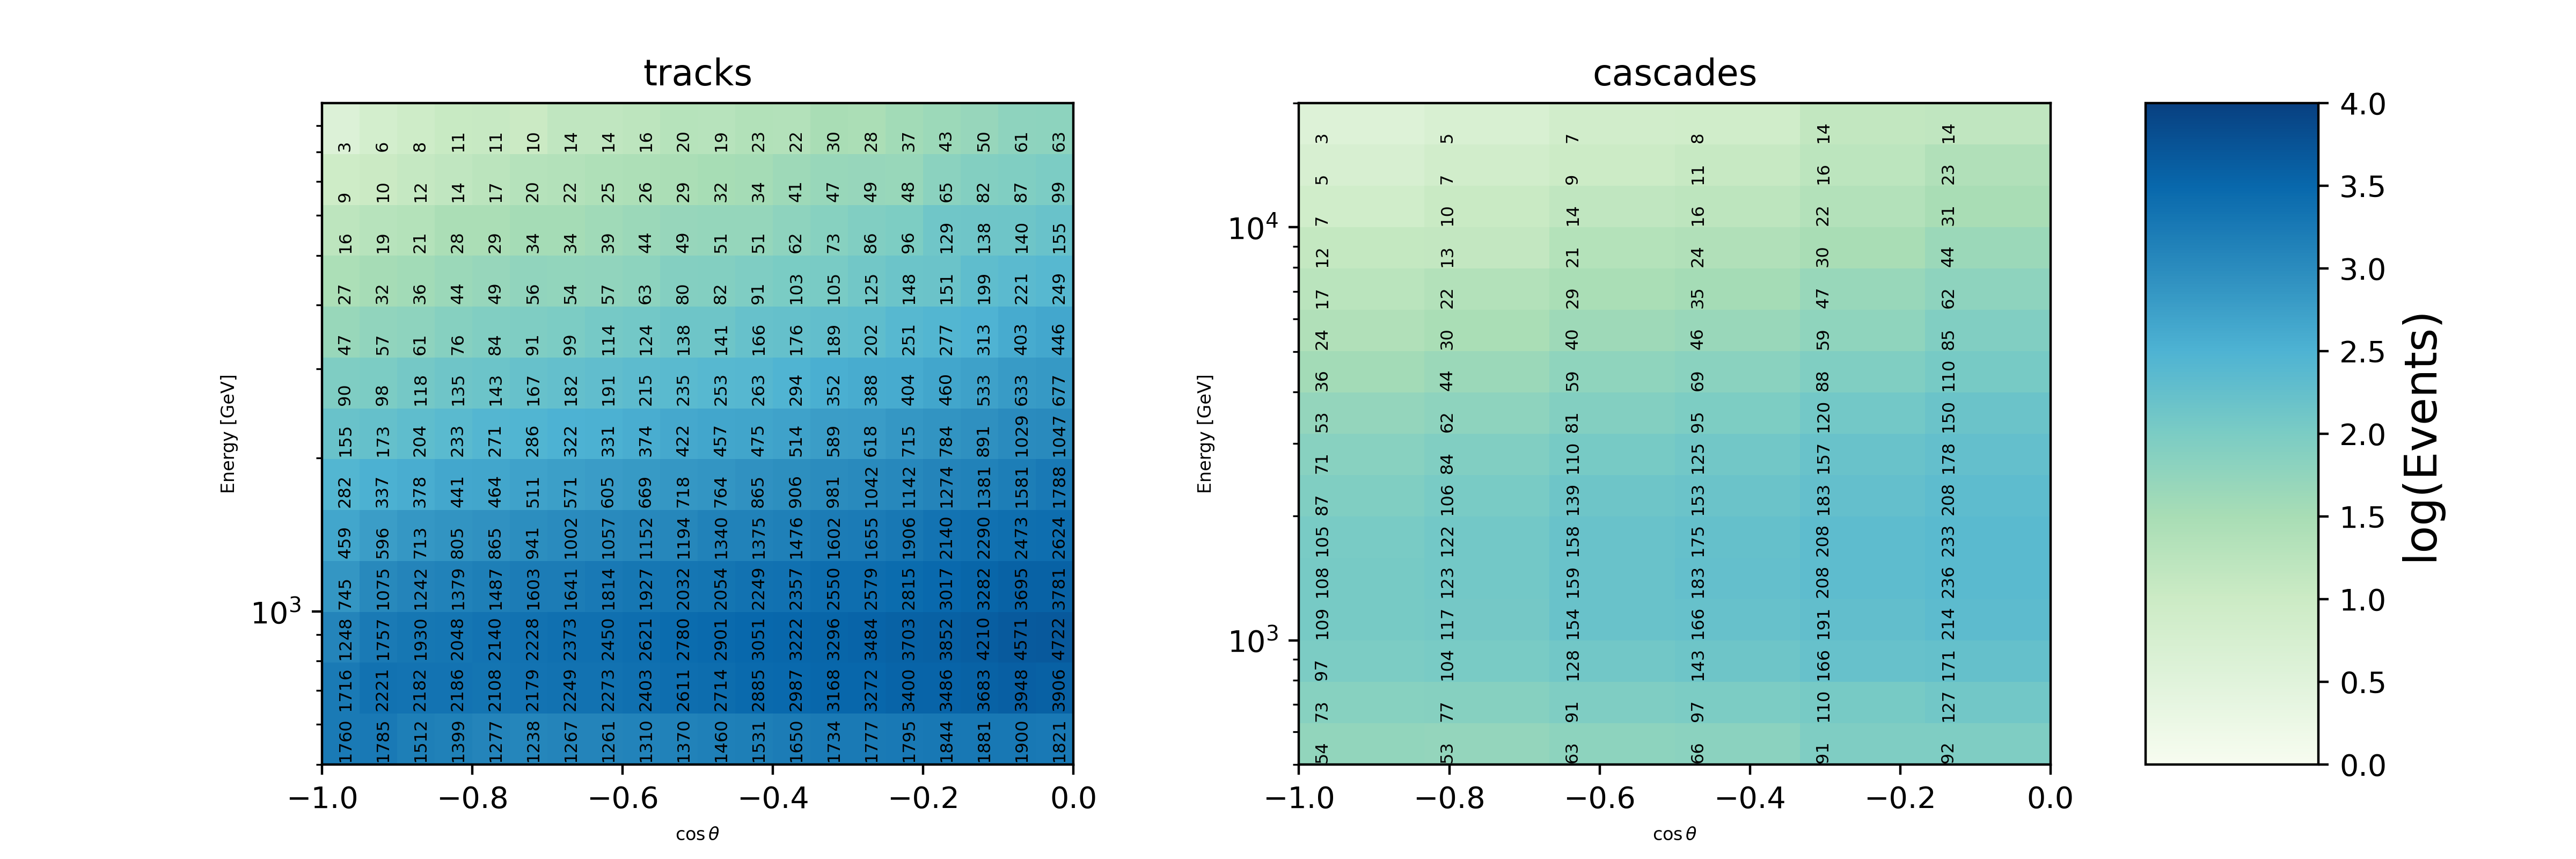
\includegraphics[width=0.8\linewidth]{figures/realization_joint.png}
    \caption{The expected numbers of events in each bin for tracks (left) and cascades (right). Assuming 7.6 years of livetime for tracks and 10 years of livetime for cascades.}\label{fig:event_no}
\end{figure}

\subsection{Cascade Event Selection}

This final level event filter was developed and published in Ref~\cite{2018PhDT17N}.

The monopod reconstruction algorithm is then run on events which survive the topological splitting cuts. 
When the reconstruction algorithm, Monopod, is run on the events surviving the level three filter described in Section SEC, 
several quantities are fit and logged including the reconstructed energy, interaction vertex, direction, and a reduced likelihood for the fit; the smaller the reduced log-likelihood is the better. 
Events for which the reduced algorithm fail, or which have a reduced log-likelihood ($rLogl$) of greater than 9.1, are discarded. 

A first series of cuts, the level four cuts, are then applied. 
These are designed to further cut away any events which are likely resulting from particles entering into IceCube. 
\begin{enumerate}
    \item Discard events which are inside the dust layer unless they are high-energy or have $rLogl<7.5$. 
    \item Discard events with a reconstructed $z$ $>500$ or $<-500$. 
    \item Discard events which are reconstructed as being near the edge, unless they are well-reconstructed $rLogl<7.6$.
    \item Discard events near the top or bottom of IceCube unless they are well reconstructed. 
    \item Discard events with very large, negative, photon delay times. 
\end{enumerate}
Large delay times are common for detector triggers resulting from uncorrelated bundles of atmospheric cosmic ray muons. 

A Boosted Decision Tree classifier is then run on the events which survive the level-four cuts. 
This BDT has been developed to classify events into three classes: cascades, hybrid, and tracks.

Events enter the cascades sample based on an energy-dependent cut on the cascade score $s_{cascade}$. Only events satisfying Equation~\eqref{eq:e_casc_cut}
\begin{equation}
    s_{\text{cascade}} > 1 - \left(\dfrac{1}{A + \exp\left[ -B(\log E_{reco} - C) \right]} + D\right),
\end{equation}\label{eq:e_casc_cut}
where the constants $A=1.539$, $B=5$, $C=4.1$, and $D=0.25$, are kept. 

\subsection{Track Event Selection}

The track sample of this analysis uses events with reconstructed energies between 500GeV and 10 TeV. 
The event selection is constructed from a series of cuts, described briefly here, and at length in References~\cite{Aartsen_2020, Aartsen_2020_prd, axani2020sterile}. % 50, 68, 69, 129

\begin{enumerate}
    \item Discard events for which fewer than fifteen DOMs are triggered or fewer than six are triggered on direct light.
    \item  For events with $0\leq\cos\theta_{\mu}^{reco}\leq 0.2$, discard if the total charge $Q_{tot}<100$ photoelectrons (PEs) or if the average weighted charge distance $<200$ meters/PE. 
    \item Remove all events with a reconstructed value of $\cos\theta_{\mu}^{reco}\geq 0.2$. This removes down-going track like events that are likely cosmic ray muons. 
    \item Discard all events with a reconstructed track length less than 200 meters, or a track smoothness $<0.6$.
\end{enumerate}

These cuts comprise the ``Golden Filter,'' described in Ref REF, and produce a sample with $\nu_{\mu}$ purity greater than 99\%. %129
An additional, ``Diamond filter,'' is used to further improve sample quality. 
It uses an additional set of cuts
\begin{enumerate}
    \item Discard events with fewer than twelve direct light DOM triggers. 
    \item Discard events with $Q_{tot}\leq20$ PE outside DeepCore. 
    \item Discard events with fifteen or fewer DOMs triggered outside DeepCore. 
    \item Discard events with $\cos\theta_{\mu}^{reco}>0.05$.
\end{enumerate}

With these event selections, we strong appearance and disappearance signatures are possible. Two possible signatures of sterile neutrino oscillations using these event samples are shown in Figure~\ref{fig:sterile_signature} in analysis space. 

\begin{figure}
    \centering
    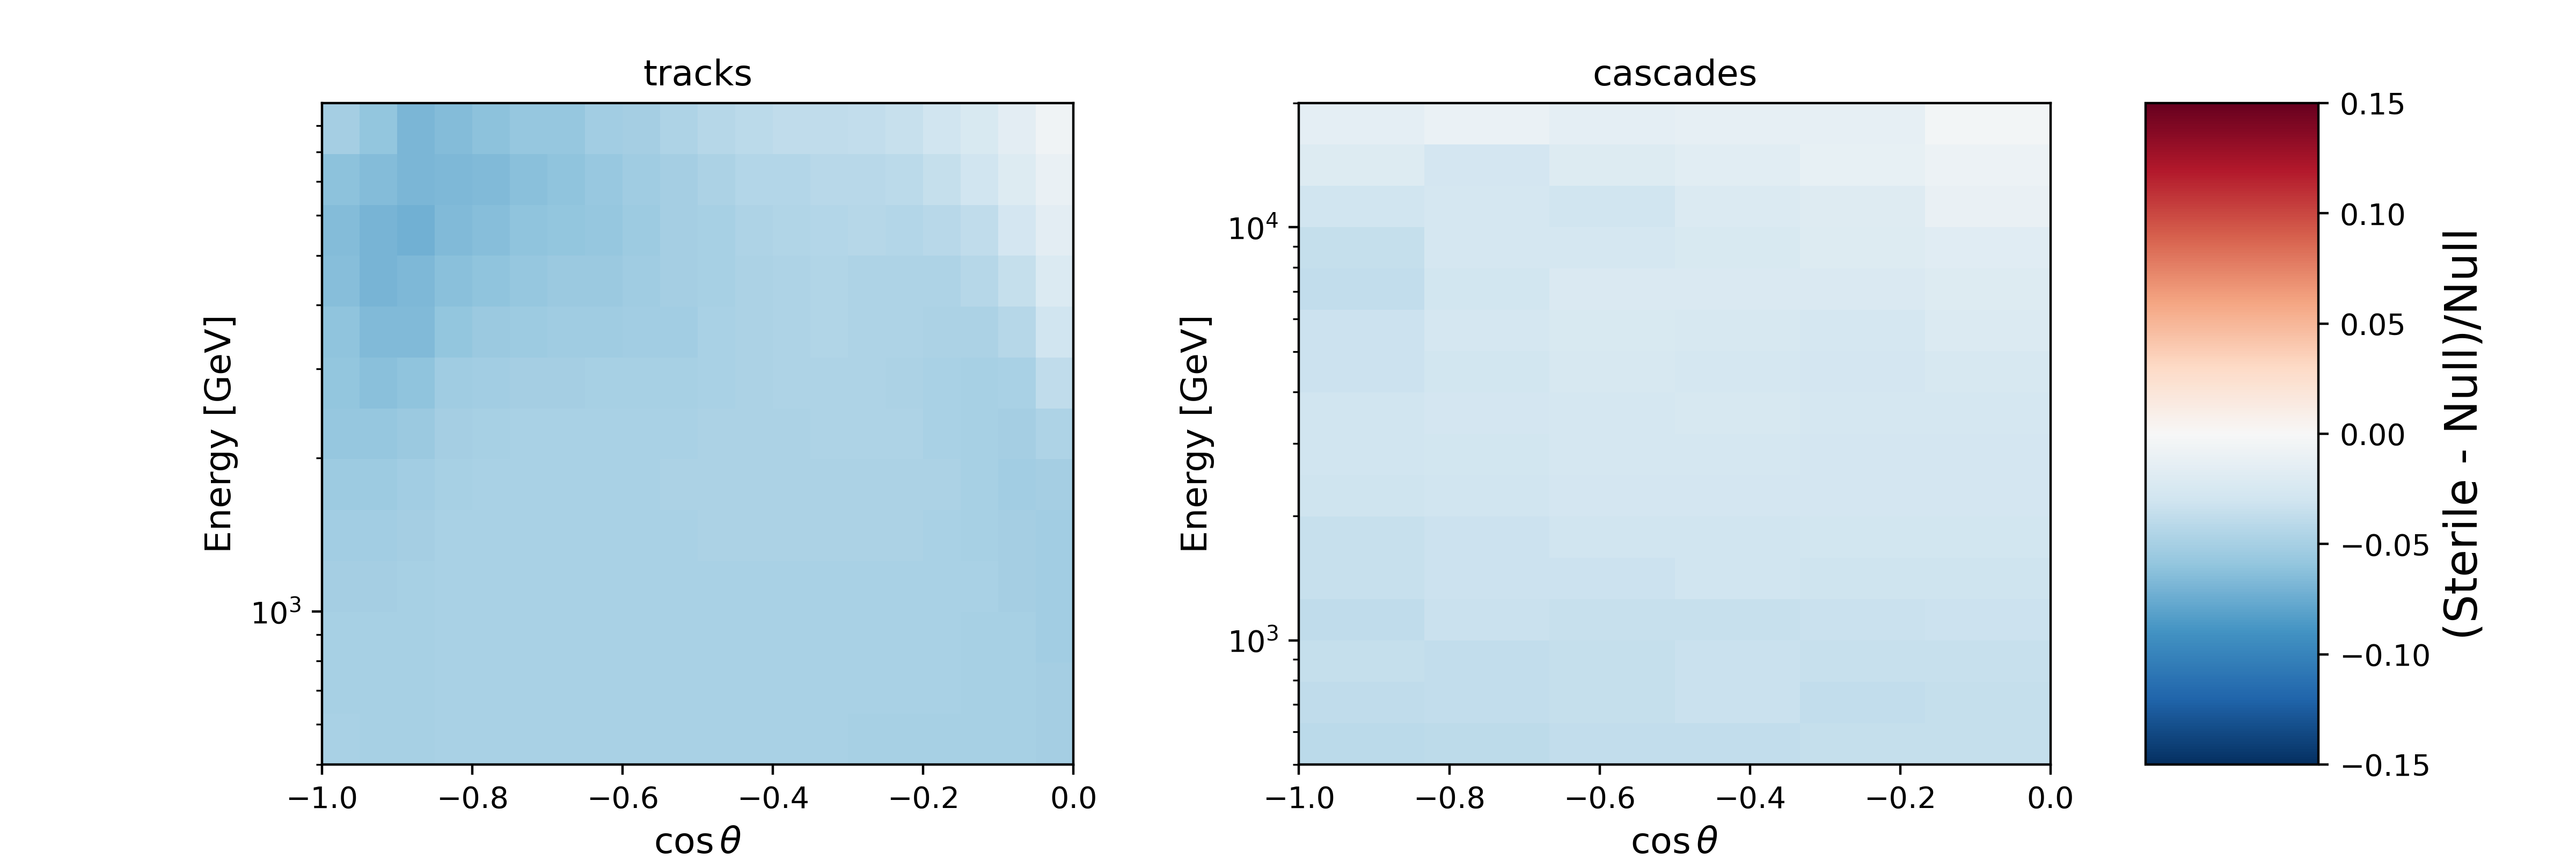
\includegraphics[width=0.45\linewidth]{figures/meows_bf_nofit.png}%
    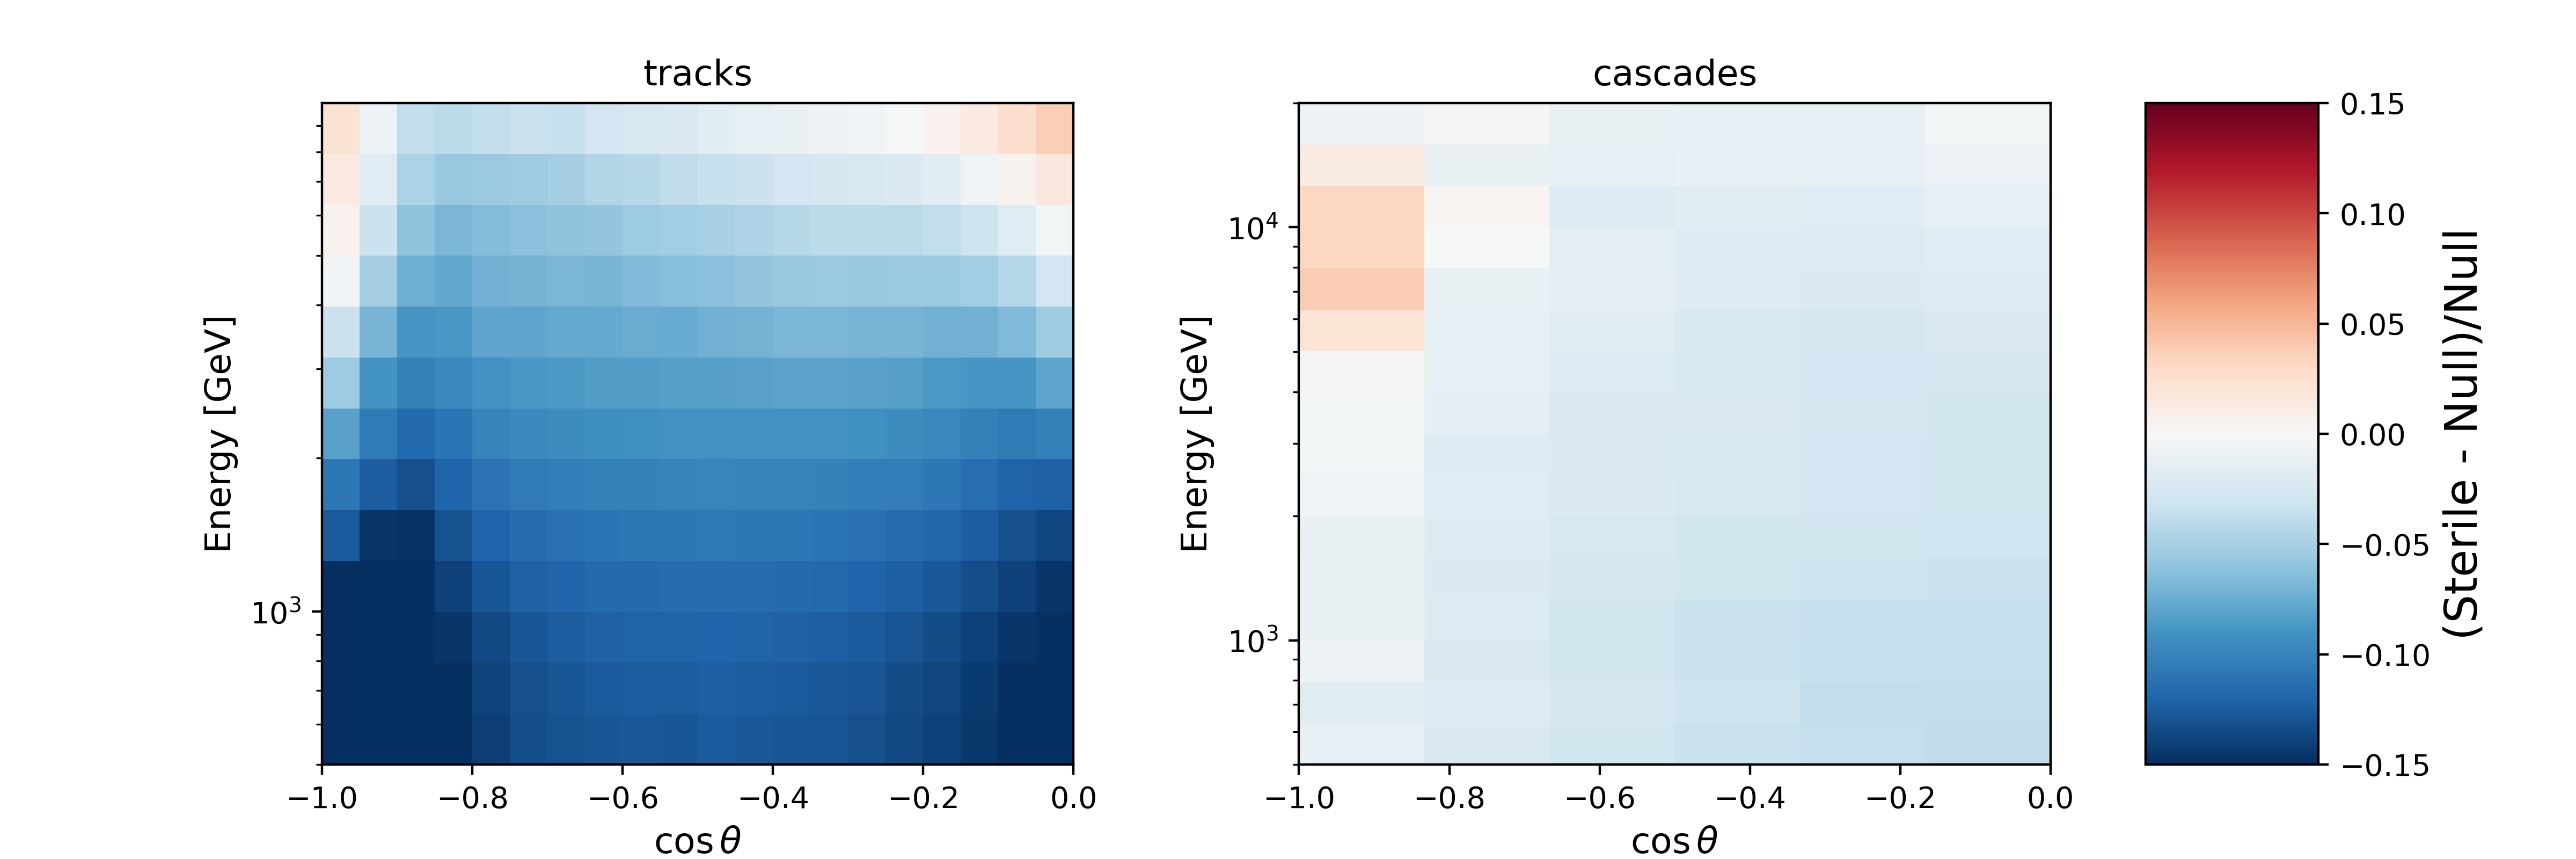
\includegraphics[width=0.45\linewidth]{figures/with_th34_nofit.png}
    \caption{Two signatures of sterile neutrinos in reconstructed space. On the left, the expected disappearance for tracks (left) and cascades (right) for a sterile neutrino model with $\sin^{2}(2\theta_{24})=0.1$ and $\Delta m_{41}^{2}=4.5$ eV$^{2}$. The same is shown on the right but with $\sin^{2}(2\theta_{34})=0.05$.}\label{fig:sterile_signature}
\end{figure}

\section{Fast Monte Carlo, Event Merging}

Approximately one thousand years of MC events were simulated for the track sample in this analysis.
This is in the ballpark of twenty-five billion events; directly reweighting all of these events for every minimizer step was found to be computationally intractable. 
To alleviate these issues, a ``Fast Monte Carlo'' algorithm was developed to merge events into meta events, which themselves would be reweighted in fits. 

Events are first weighted according to a flux hypothesis, and the contributions to an event's conventional, prompt, and astrophysical weight are all calculated and stored separately. 
Events are then binned, in reconstructed quantities, into a fine grid whose bin widths are a fraction of the normal analysis bin widths; this fraction is defined as the \textit{fastmode scaling}.
As an example, a fastmode scaling of 0.5 would use twice as many bins along each fit axis, and a scaling of 0.1 would use 10 times as many bins along each fit axis. 


Events within each of these fine bins are then merged into meta-events; the separate flux-weights are added directly, and a weighted-average is done for analysis quantities like energy and zenith.
The weighted average is calculated according to Equation~\eqref{eq;weighted_fm} for analysis quantity $A$ in fastmode bin $\alpha$.
\begin{equation}\label{eq;weighted_fm}
A_{meta}^{\alpha} = \dfrac{\sum_{i}^{n} A_{\alpha, i} \left(w_{\alpha, i}^{conv} + w_{\alpha,i}^{prompt} + w_{\alpha,i}^{astro}\right) }{\sum_{i}^{n} \left(w_{\alpha, i}^{conv} + w_{\alpha,i}^{prompt} + w_{\alpha,i}^{astro}\right)}
\end{equation}
The sum is carried out over all $n$ events in a fastmode bin. 
These meta-events are then saved with their summed flux-weights and weighted-average analysis quantities.
This procedure is carried out for each tested physics hypothesis, although it is only applied to the track sample. 
A fastmode scaling of 0.1 was used in this analysis and values smaller than 0.25 have been found to produce stable results. 


\section{Likelihood Metric}\label{sect:llh_metric}

The likelihood used in this analysis is defined as the probability of observing a given set of data, or pseudo-data, assuming some physics hypothesis.
It is quantified as 
\begin{equation}
    \mathcal{L}(\vec{\Theta}, \vec{\eta}) = \prod_{i=0}^{\text{bins}} \mathcal{L}_{eff}\left( w_{i}^{sum}, w_{2,i}^{sum}, k_{i} \right),
\end{equation}
where $w_{i}$ and $w_{2,i}$ are the sums of the MC weights and MC weights squared, respectively, in bin $i$; $k_{i}$ is the observed number of events (or pseudo-events). 
$\vec{\Theta}$ is the tested physics hypothesis and $\vec{\eta}$ the set of nuisance parameters. 

The effective likelihood function, defined in Ref~\cite{effective_llh}, is part of a family of likelihood metrics used to account for MC statistical uncertainty. 
We use the form where
\begin{align}
    \alpha&=\dfrac{\mu^{2}}{\sigma^{2}} +1 & &\text{and} & \beta&=\dfrac{\mu}{\sigma^{2}}.
\end{align}
Since each simulated MC event is just one event, $\mu = w_{i}$ and $\sigma^{2} = w_{2,i}$\footnote{MC events are merged into into `meta-events' to speed up reweighting, where the functional forms are slightly more complicated}, and
\begin{equation}
    \mathcal{L}_{eff}(\vec{\Theta} | k) = \left(\dfrac{\mu}{\sigma^{2}}\right)^{\tfrac{\mu^{2}}{\sigma^{2}} + 1} \Gamma\left(k + \dfrac{\mu^{2}}{\sigma^{2}} + 1\right) \left[ k! \left(1+\dfrac{\mu}{\sigma^{2}}\right)^{k+\tfrac{\mu^{2}}{\sigma^{2}} + 1} \Gamma\left(\dfrac{\mu^{2}}{\sigma^{2}} +1\right)\right]^{-1}
\end{equation}
where $\Gamma$ is the gamma function. 

The set of nuisance parameters describe that describe systematic uncertainties are themselves constrained by Gaussian priors functions. 
These priors are used to weight the likelihoods, which is maximized to form a profile likelihood, defined as 

\begin{equation}
\mathcal{L}_{\text{profile}}\left(\vec{\theta}\right) = \text{max}_{\vec{\eta}}\left[\mathcal{L}(\vec{\Theta}, \vec{\eta}) \Xi(\vec{\eta}) \right]
\end{equation}
where $\Xi(\vec{\eta})$ is the total likelihood penalty for the set of nuisance parameters $\vec{\eta}$ calculated accounting for the correlations between the priors. 

We then construct an analysis test statistic (TS) for producing confidence intervals, which we define as 
\begin{equation}\begin{split}
TS(\vec{\Theta}) &= -2\left[ \log\mathcal{L}_{\text{profile}}(\vec{\theta}) - \log\mathcal{L}_{\text{profile}}(\vec{\Theta}_{min}) \right] \\
&= -2 \Delta \log\mathcal{L}_{\text{profile}}(\vec{\theta})\\
&=-2\Delta \text{LLH}
\end{split}\end{equation}
where $\vec{\Theta}_{min}$ is the sterile hypothesis that maximizes the likelihood, and best matches the data: the best fit point. 

\textit{Short discussion about biases introduced by this likelihood function}

\section{Tests}

A series of tests were performed to validate the implementation of the nuisance parameters and verify the performance of the fitting framework. 

\subsection{Previous Results Cross-Check}

Using only the track sample, we verified we were able to recover similar sensitivities to the original eight-year sensitivity published in References~\cite{Aartsen_2020} and~\cite{Aartsen_2020_prd}. 
First, a comparison was done using the older GolemFit framework and the new PISA framework~\cite{pisa} using the same exact nuisance parameter implementations and fluxes. 
The sensitivities, calculated at 90\% C.L. and for two degrees of freedom, for both GolemFit and PISA are shown in Figure~\ref{fig:comparison} (left).

Then, additional fluxes, gradients, and Fast MC, were generated in logarithmic steps in $\sin^{2}(2\theta_{14})$ and $\Delta m_{41}^{2}$ space.
Using the new nuisance parameter implementations and Daemonflux gradients, we evaluated the same 90\% CL sensitivities for two degrees of freedom.
The resulting sensitivities are shown in Figure~\ref{fig:comparison} (right) with the previous sensitivities overlain. 
As mentioned in Section~\ref{sec:daemon_sense}, the observed sensitivities using DaemonFlux are worse than the older 8-year sensitivities. 

As a means of verifying suspicions that the charge-ratio is responsible for the hit to the expected sensitivity. I now will write about the check where I made the charge ratio smaller 

\begin{figure}
    \centering
    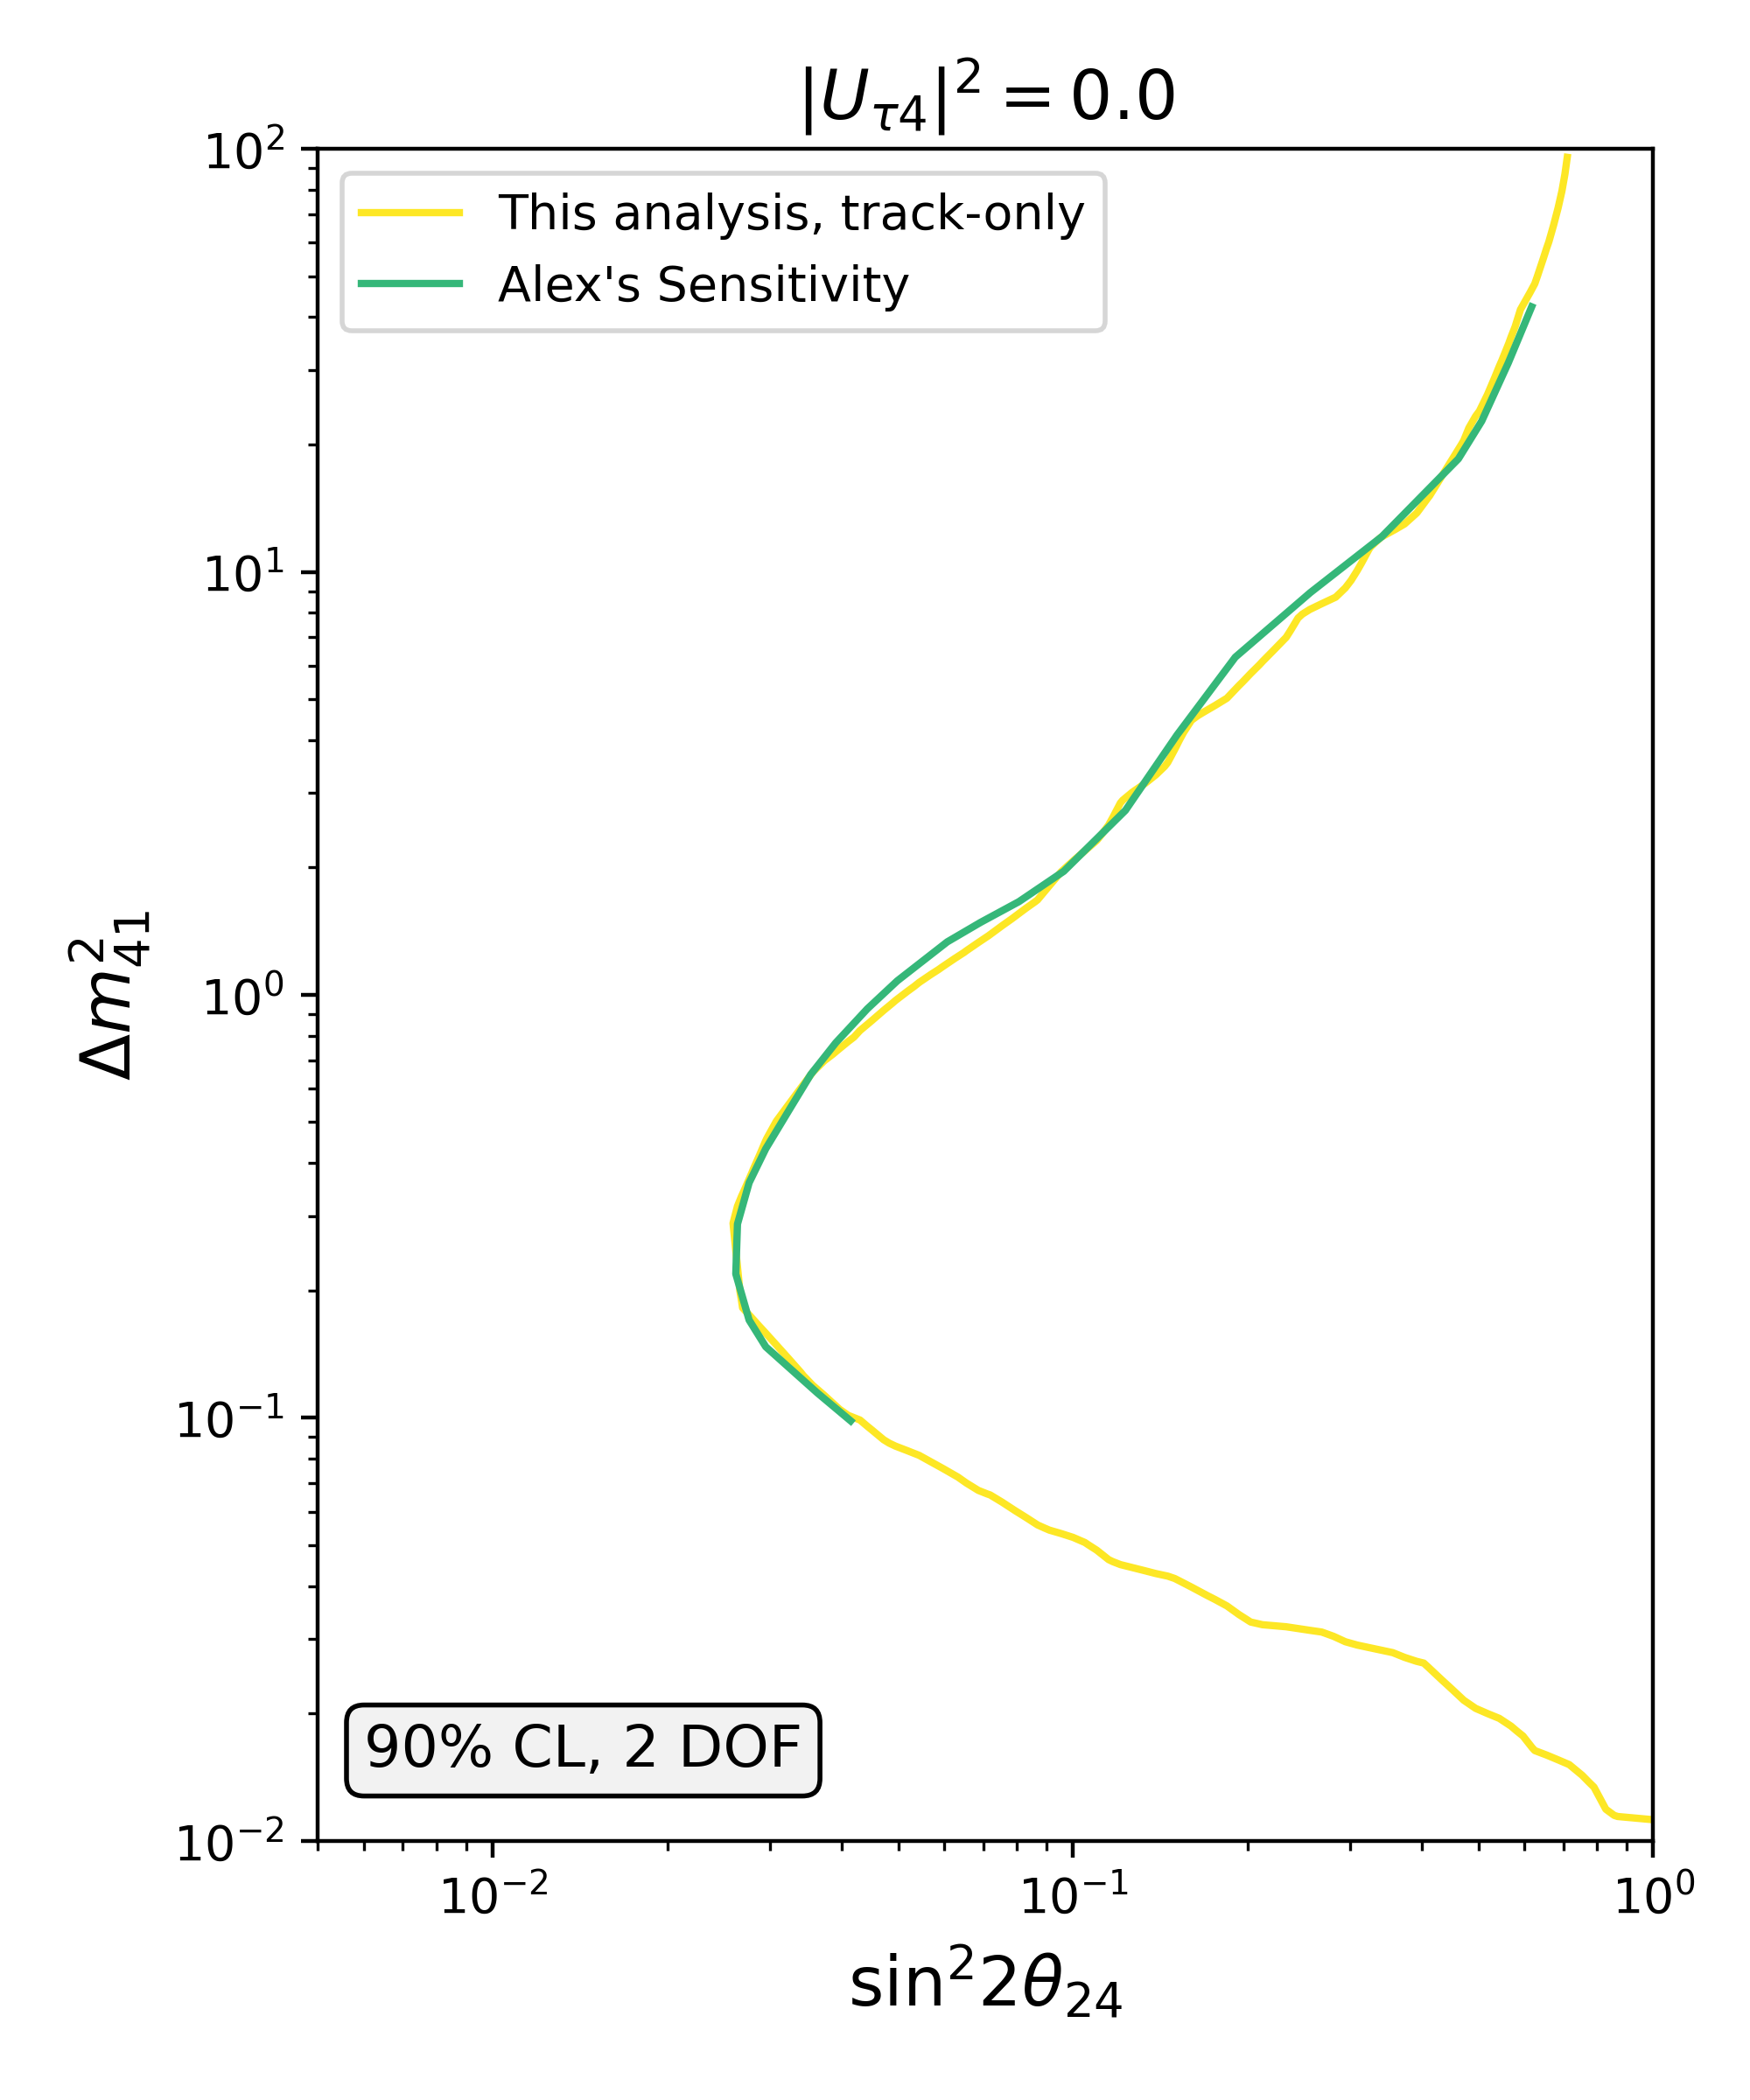
\includegraphics[width=0.6\linewidth]{figures/track_asimov_oldairs_Realization_Asimov_sterile_0_cl0.9_dof2.png}
    \caption{The 90\% CL sensitivity contours for two degrees of freedom, using only the track sample, as determined for this analysis (yellow) and the original 8-year tracks sample (green).}\label{fig:comparison}
\end{figure}

\subsection{Inject-Recover Systematic Tests}

Pseudo-experimental results, or `realizations,' are first calculated by perturbing all nuisance parameters within their priors, simultaneously, and getting the expected event rates without additional statistical variation applied. 
Fits are then carried out to each of these realizations.

The results are tabulated below in two figures: in Figure~\ref{fig:ir_nopriorpert} the results are shown where the priors on the nuisance parameters are left at their original value, and in Figure~\ref{fig:ir_priorpert} the priors are changed to the value of the injected nuisance parameter. 
In Figure~\ref{fig:ir_priorpert}, the injected values are all recovered. 

In Figure~\ref{fig:ir_nopriorpert}, the flatter the trend is then the more tightly-constrained its prior is compared to the shape effects caused by the nuisance parameter itself. 
Conversely, parameters which recover injected
The cross section uncertainty and Barr-Z parameters are observed to have a minor effect on the fitting. 

\begin{figure}
    \centering 
    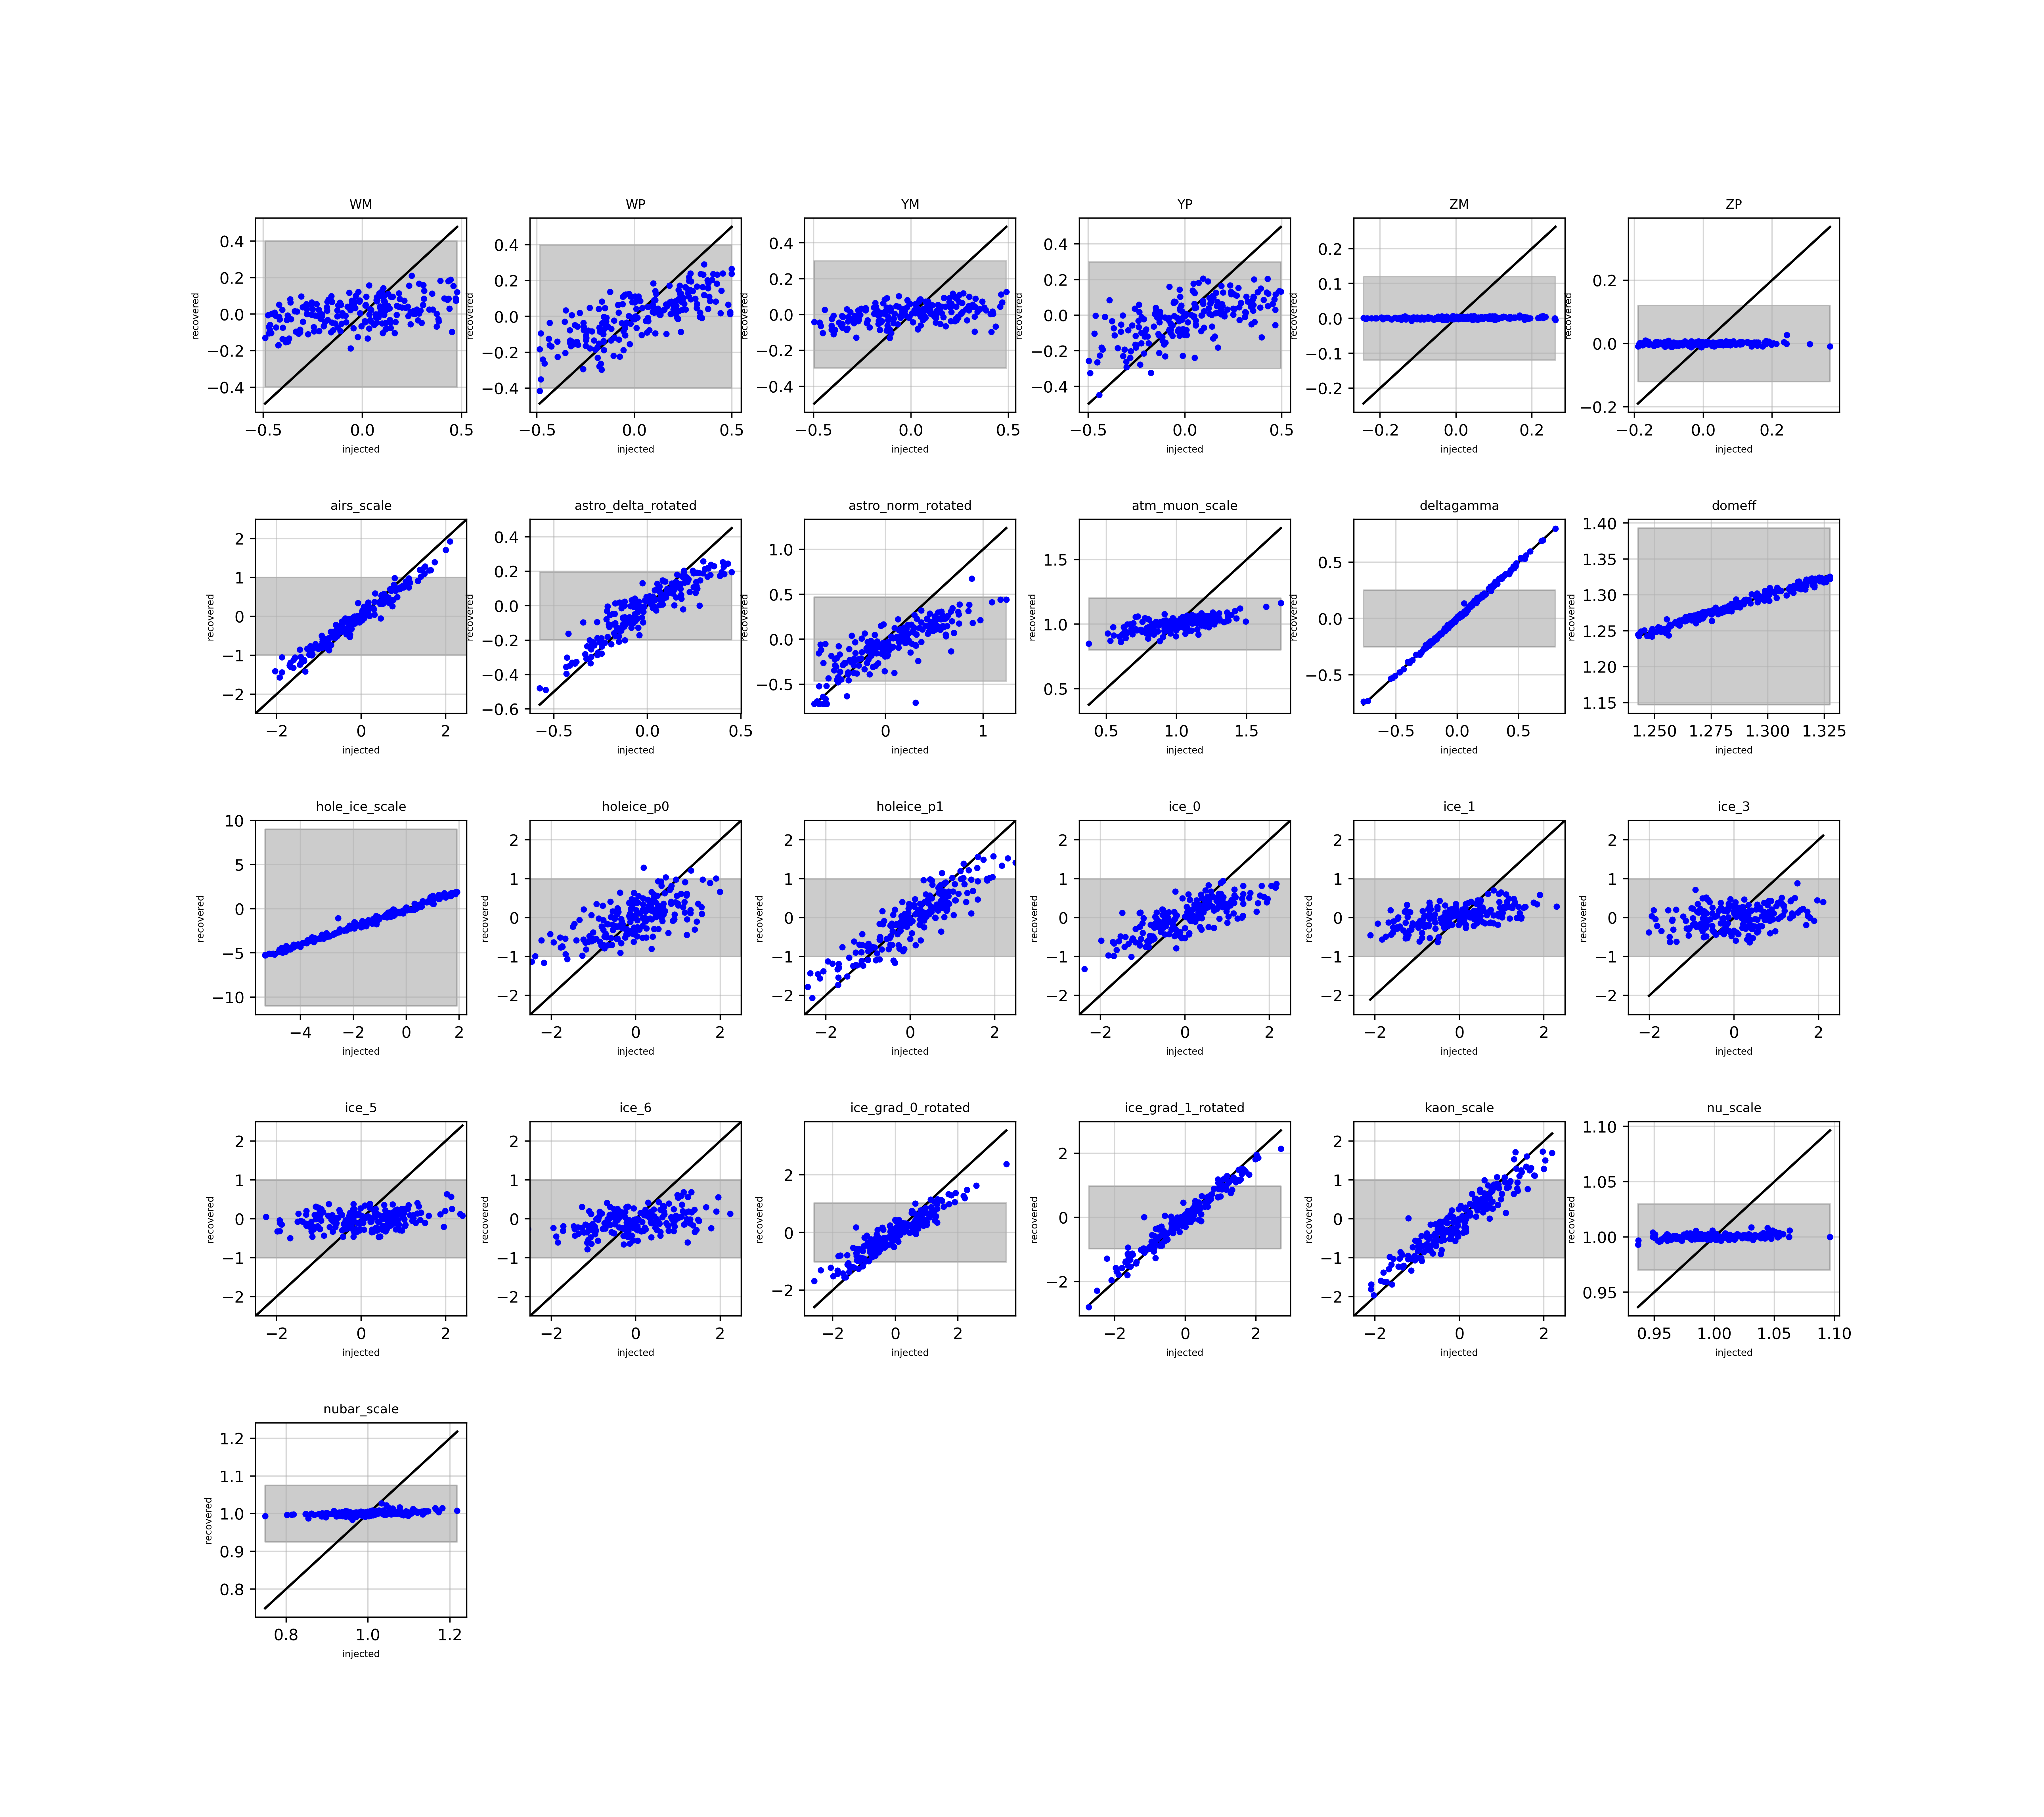
\includegraphics[width=0.7\linewidth]{figures/syst_ir_shuffle_nofix.png}
    \caption{Fit results after injecting various perturbed values for each nuisance parameter and running the fitter. A shaded gray region demonstrates the $1\sigma$ prior width on the nuisance parameter's prior.}\label{fig:ir_nopriorpert}
\end{figure}


\begin{figure}
    \centering 
    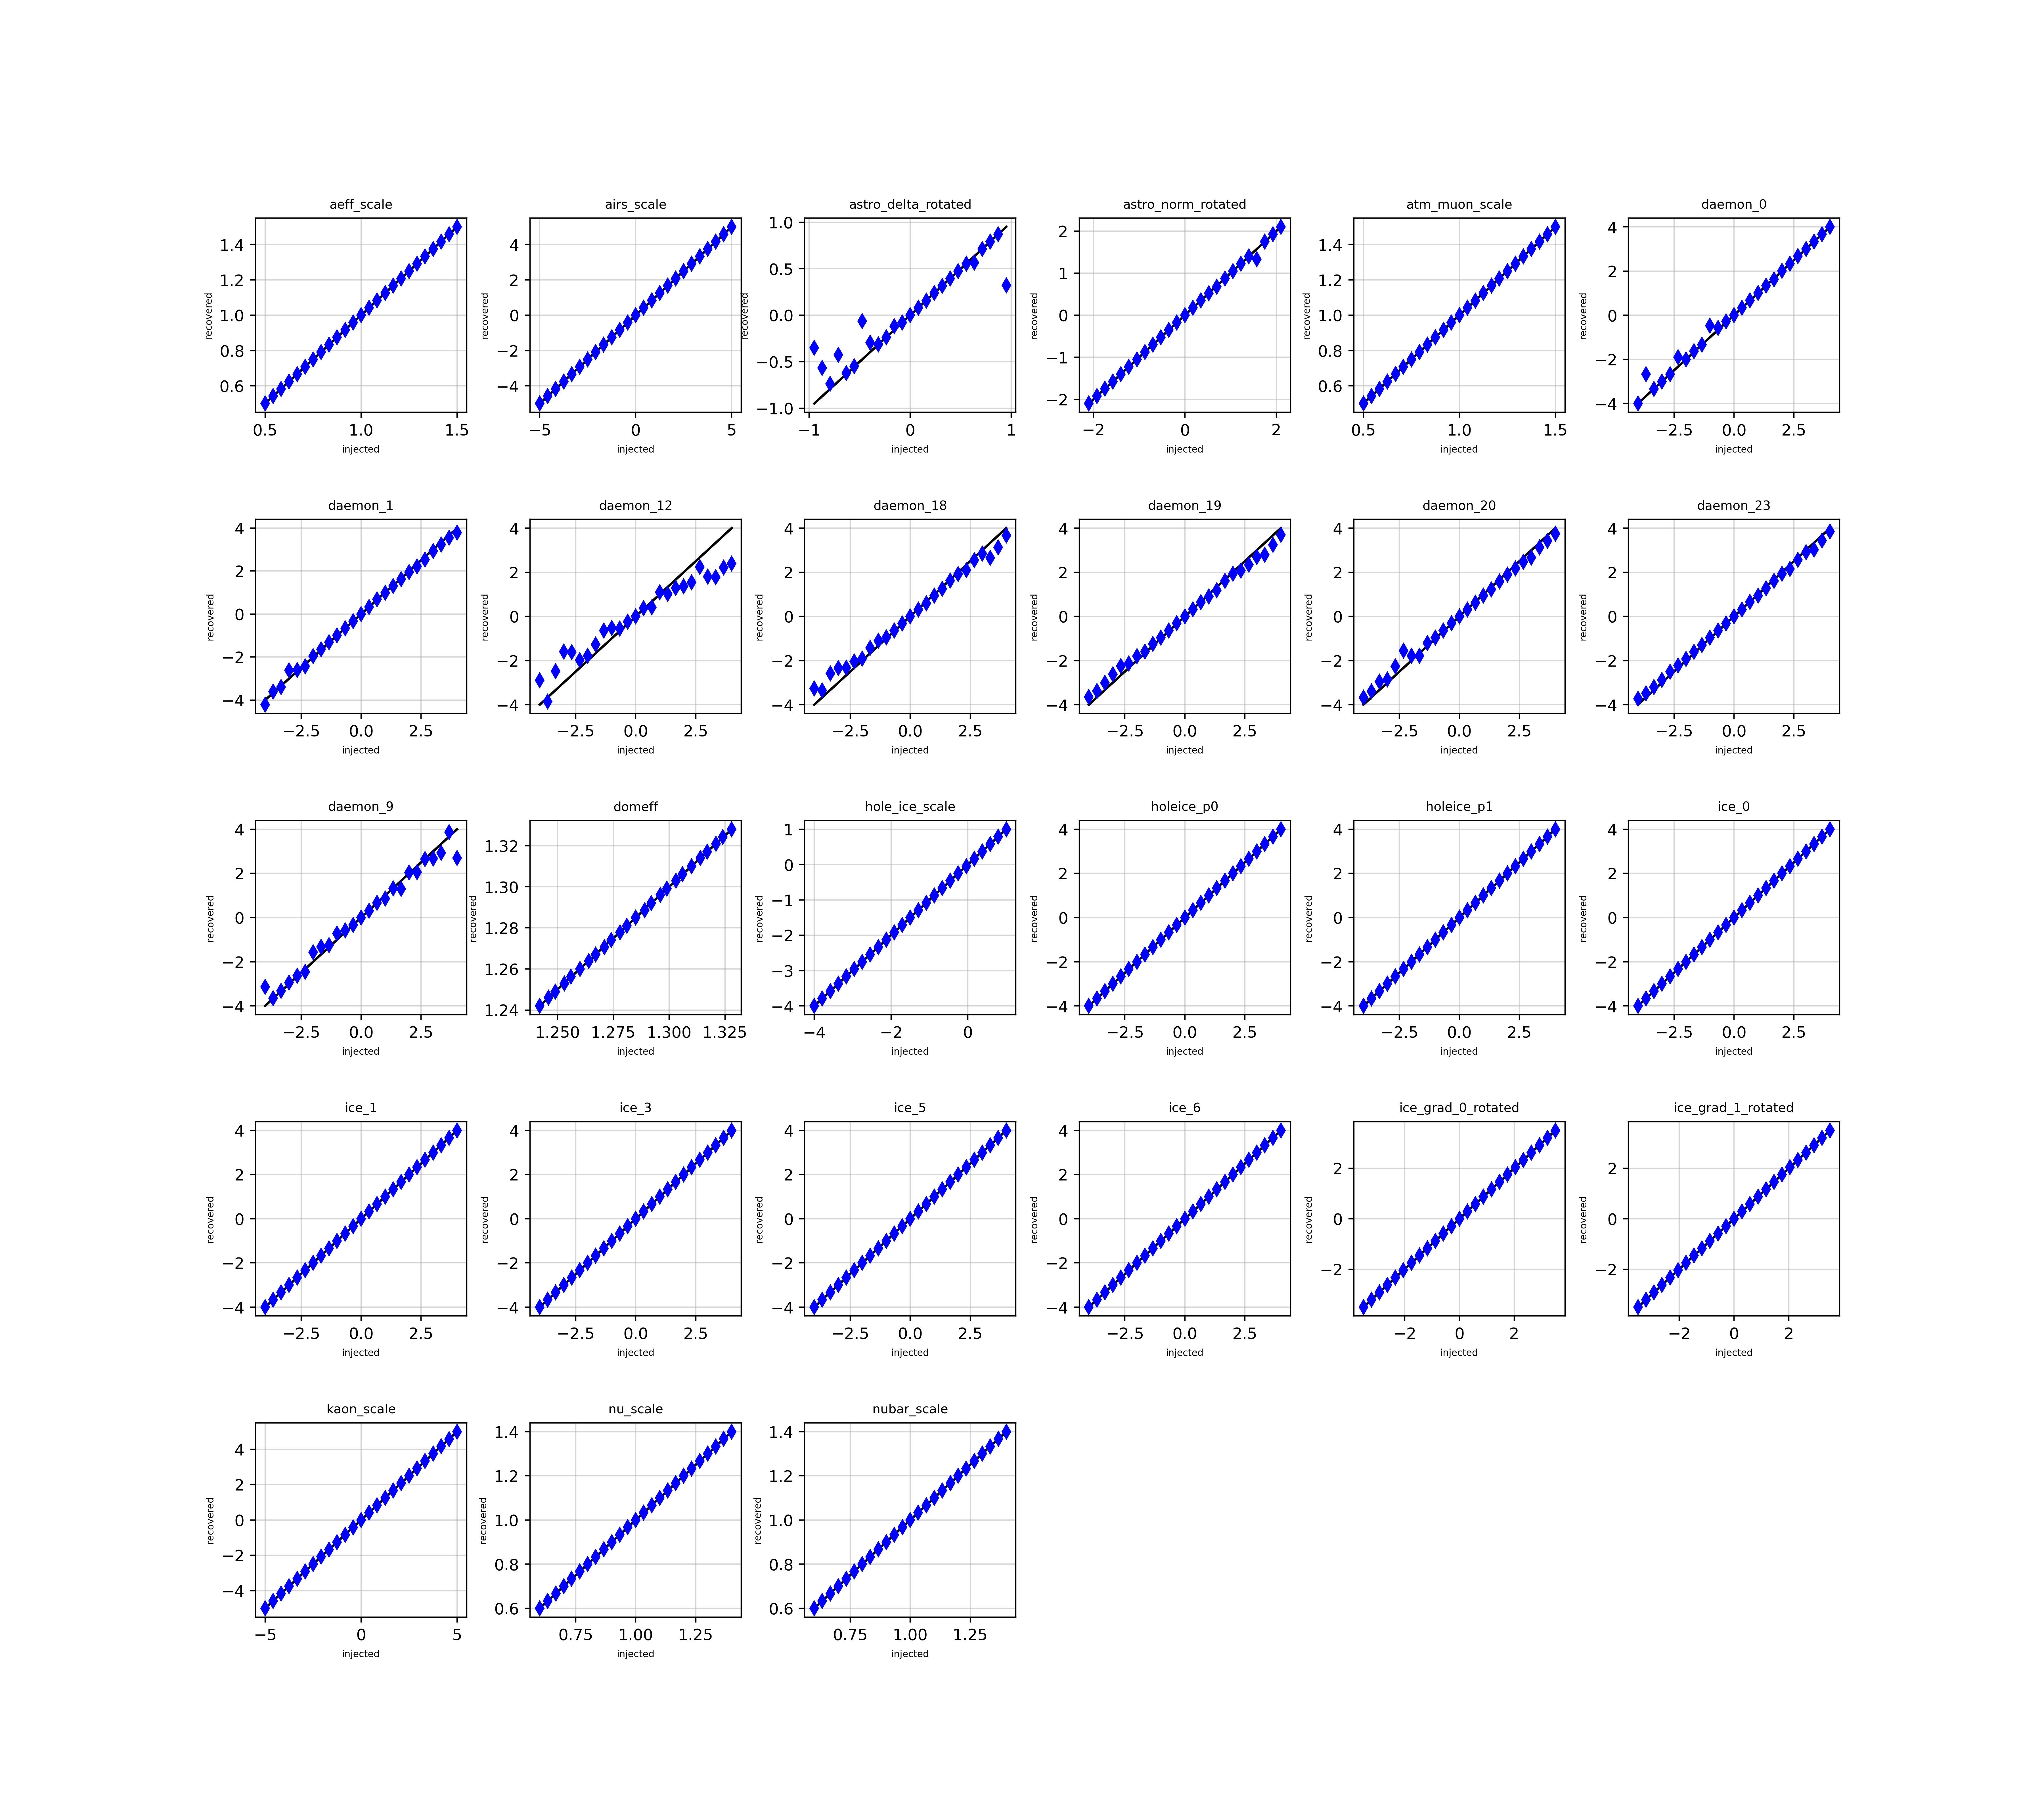
\includegraphics[width=0.7\linewidth]{figures/update_inject_recover_syst_prior.png}
    \caption{Fit results after injecting various perturbed values for each nuisance parameter and running the fitter. Priors are adjusted in each fit according to the injected values.}\label{fig:ir_priorpert}
\end{figure}

\subsection{Asimov Sensitivity}

First, a single realization was generated without applying statistical variation on the per-bin expectation. 
This is the Asimov realization. 
Fits were performed for this simulated observation and test scores were calculated for each one following the metrics defined in Section~\ref{sect:llh_metric}.
The 90\% confidence level $\chi^{2}$ threshold was calculated for three degrees of freedom for the fit scan, and the resulting sensitivity contours are shown in Figure~\ref{fig:asimov_sense}. 
These results are plotted, superimposed against other experiment's sensitivities, in Figure~\ref{fig:asimov_compare}. 
Sensitivities are compared at 90\% confidence level and assuming two degrees of freedom $\Delta m_{41}^{2}=$ 1.0 eV$^{2}$.

The sensitivities here are observed to be worse than those predicted earlier in Chapter~\ref{chapter:sense}, though this is not surprising; here a full treatment of systematic uncertainty is used.
In addition to this, the newer flux model predicts a higher charge ratio, resulting in fewer signal-neutrinos from being apparent against the $\nu_{\mu}$ flux.

\begin{figure}
    \centering
    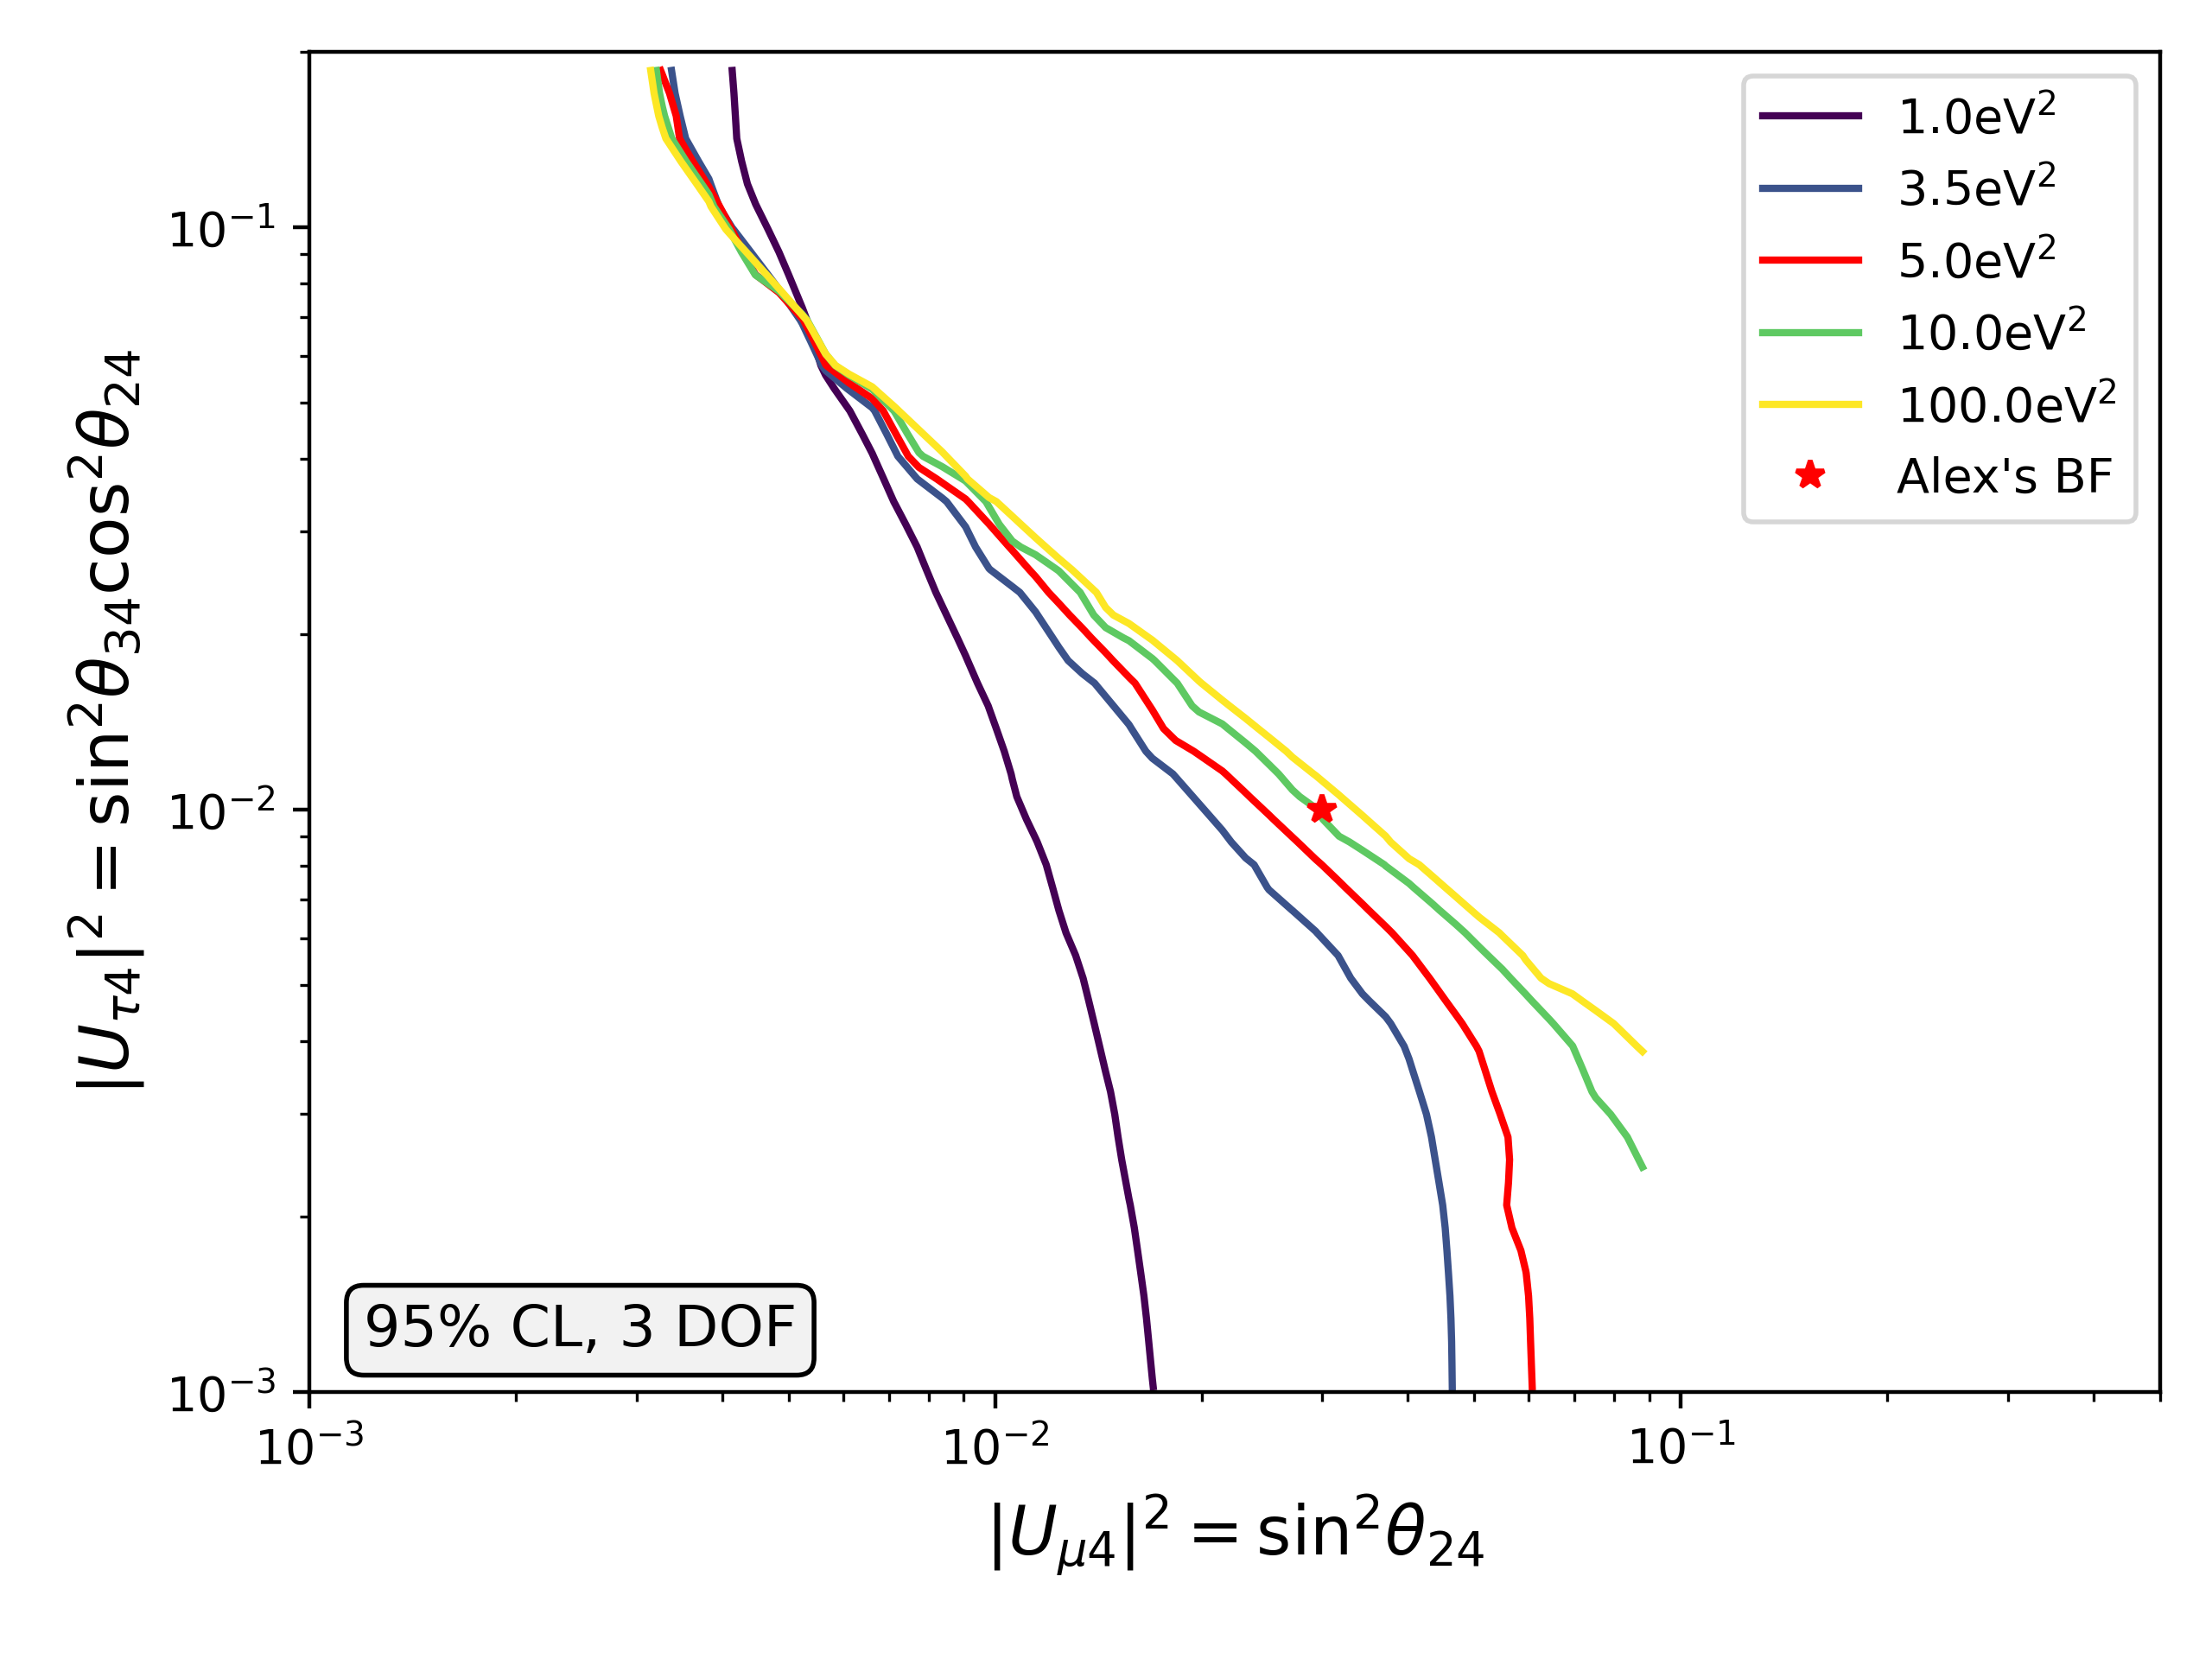
\includegraphics[width=0.7\linewidth]{figures/joint_asimov_oldairs_Realization_Asimov_sterile_0_cl0.95_dof3}
    \caption{The 90\% confidence level sensitivity contours with three degrees of freedom for this analysis.}\label{fig:asimov_sense}
\end{figure}

\begin{figure}
    \centering
    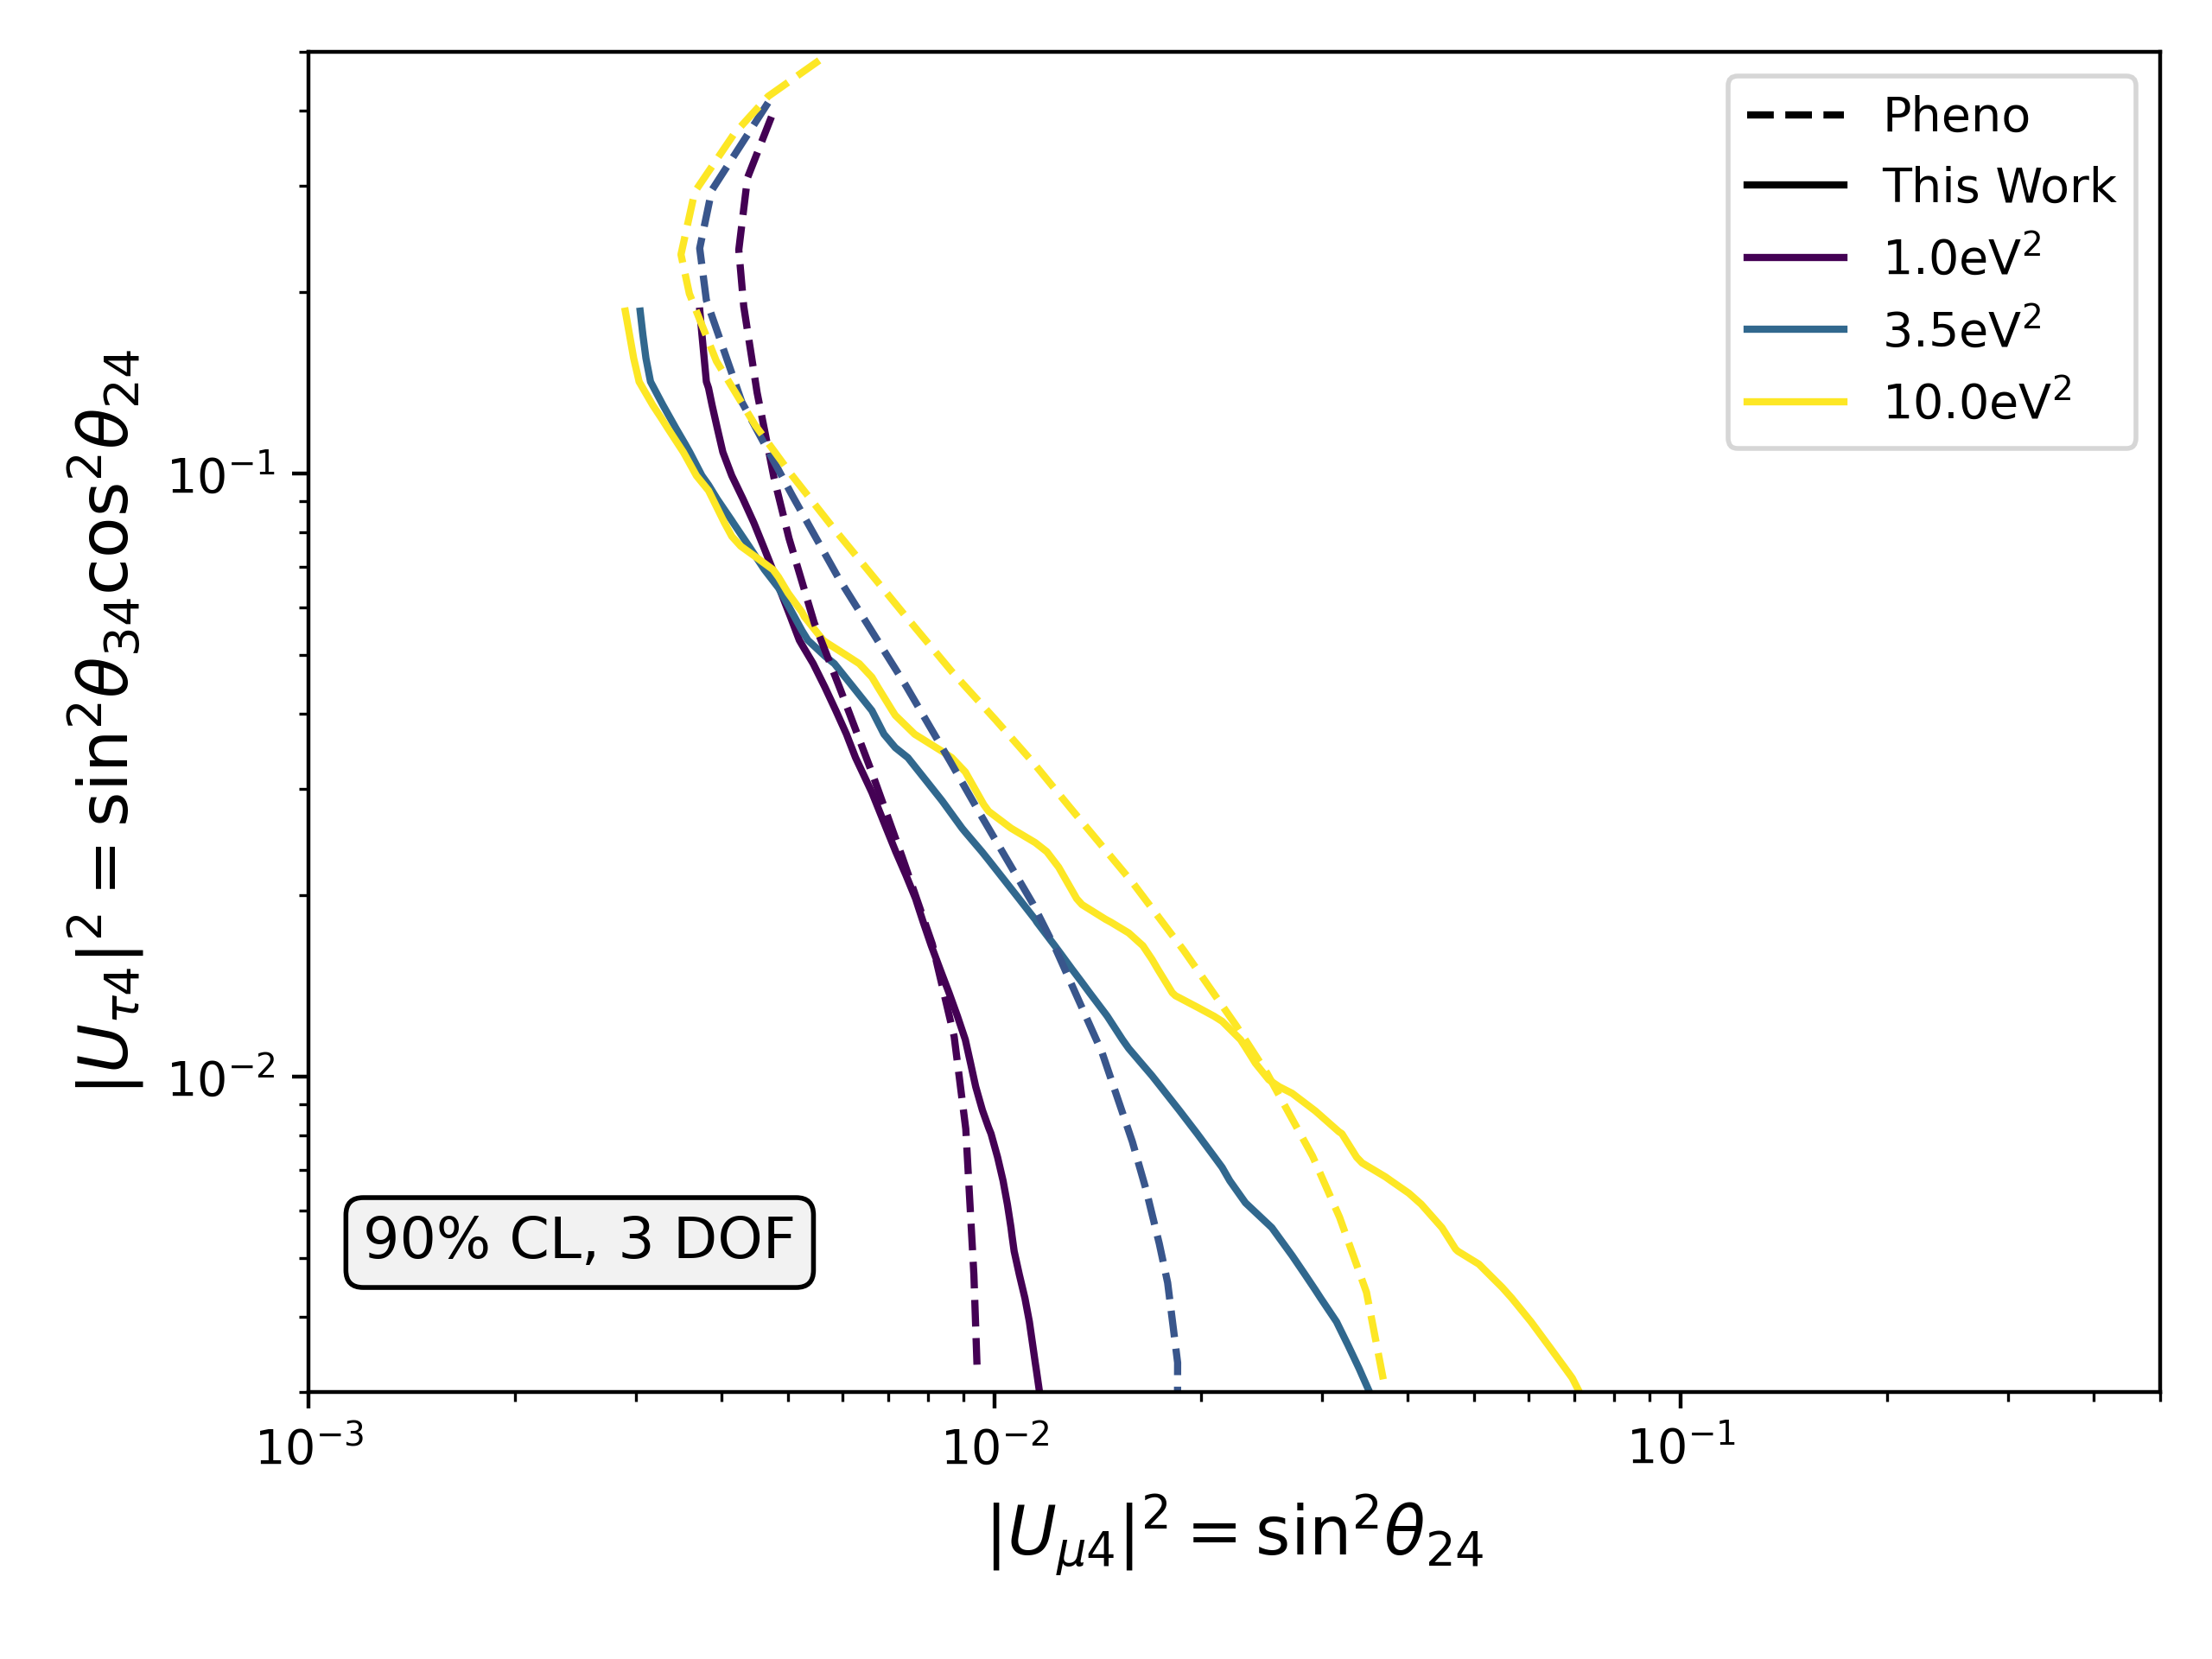
\includegraphics[width=0.45\linewidth]{figures/pheno_joint_asimov_oldairs_Realization_Asimov_sterile_0_cl0.9_dof3.png}%
    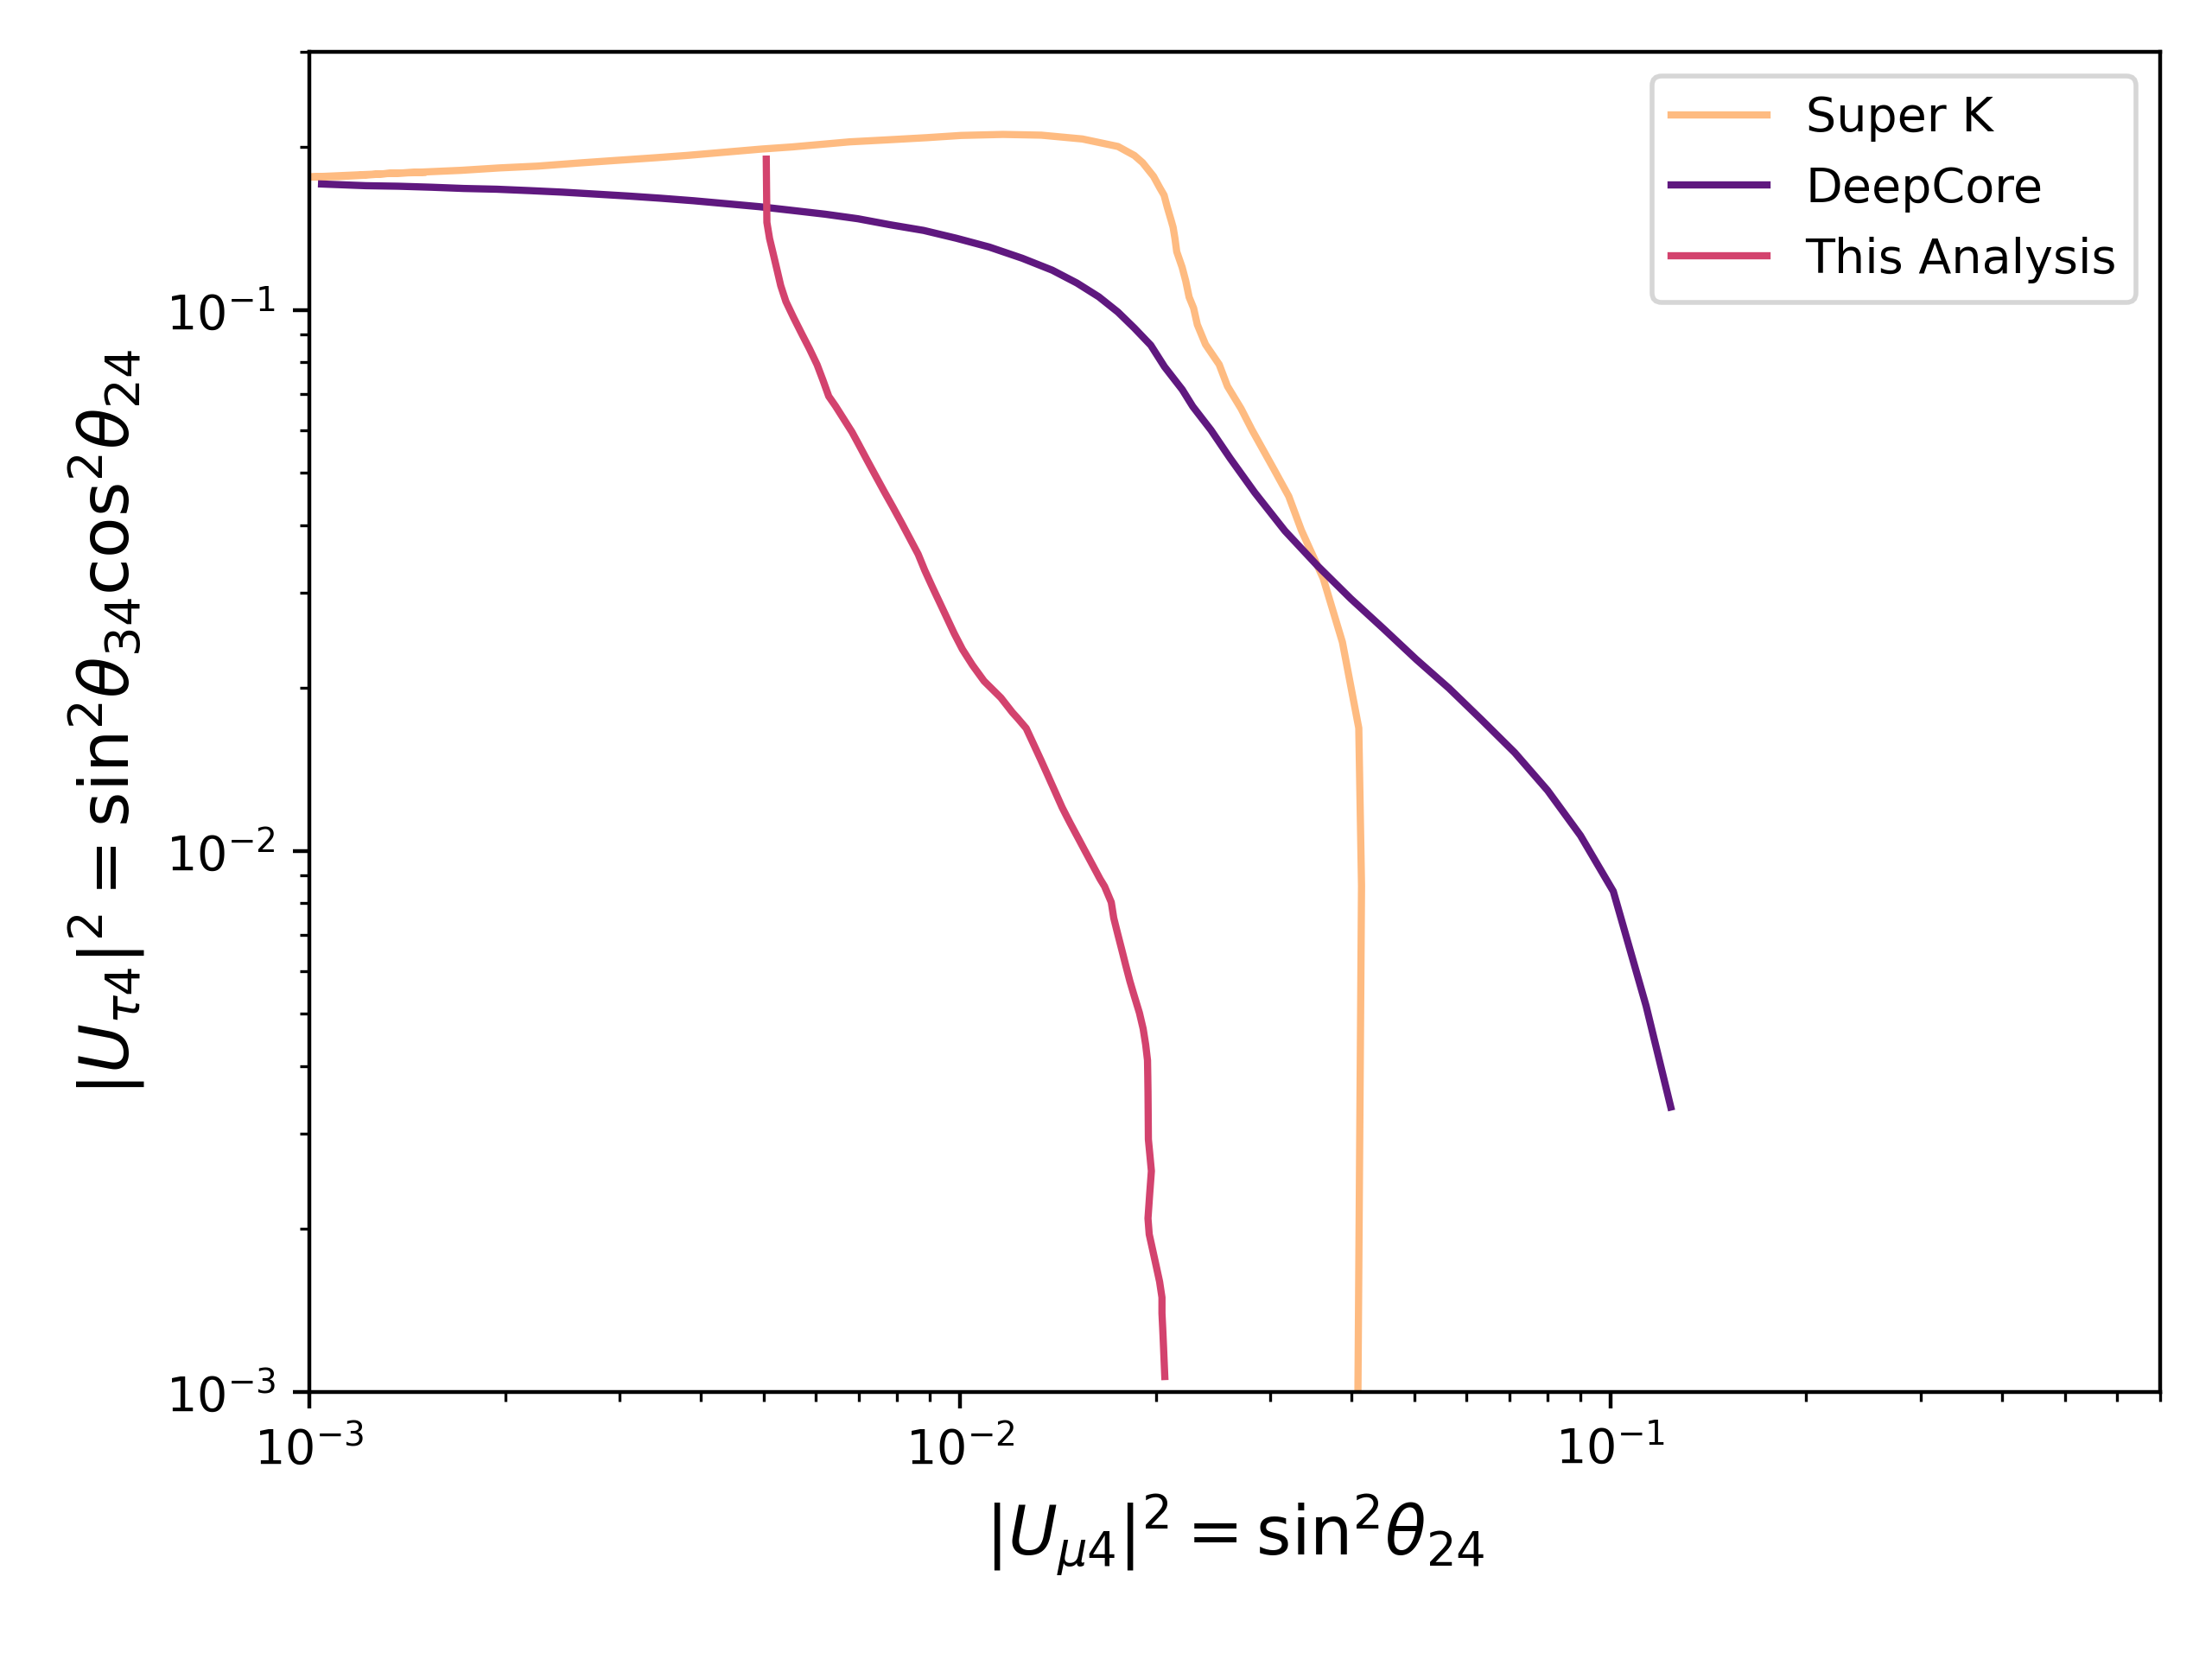
\includegraphics[width=0.45\linewidth]{figures/comparison.png}
    \caption{The 90\% confidence level sensitivity contours for this analysis with two degrees of freedom at $\Delta m_{41}^{2}=$ 1.0 eV$^{2}$ (left), and  4.5 eV$^{2}$ (right), are shown. Senstivities from DeepCore~\cite{Aartsen_2017_dc} and Super-K~\cite{PhysRevD.91.052019} at 1.0eV$^{2}$ are also shown.}\label{fig:asimov_compare}
\end{figure}


\subsection{Systematic Impact Tests}

Nuisance parameters were collected into ``bundles.'' 
Asimov sensitivity scans~\cite{Cowan_2011} were then performed for each bundle while fixing the parameters of that bundle to their central values.
The resulting confidence intervals then show the impact of fixing those nuisance parameters. 
The bundles are 
\begin{enumerate}
    \item Conv(entional): Daemonflux~\cite{yanez2023daemonflux} parameters, AIRS scale, and the kaon-nucleon cross section uncertainty
    \item Astr: astrophysical normalization and the spectral index
    \item Det(ector): hole ice uncertainty, DOM efficiency, and the bulk-ice uncertainty
    \item Muon: the CR muon background\footnote{Because of the large, extra, error introduced by the muon background, for this systematic impact test a special realization is generated and fit to where there no muon contribution is added at all.}
    \item (Norm)alization: everything is fixed except for the normalization.
\end{enumerate}
These sensitivity contours are shown at 90\% confidence level and with three degrees of freedom in Figure~\ref{fig:impact}

\begin{figure}
    \centering
    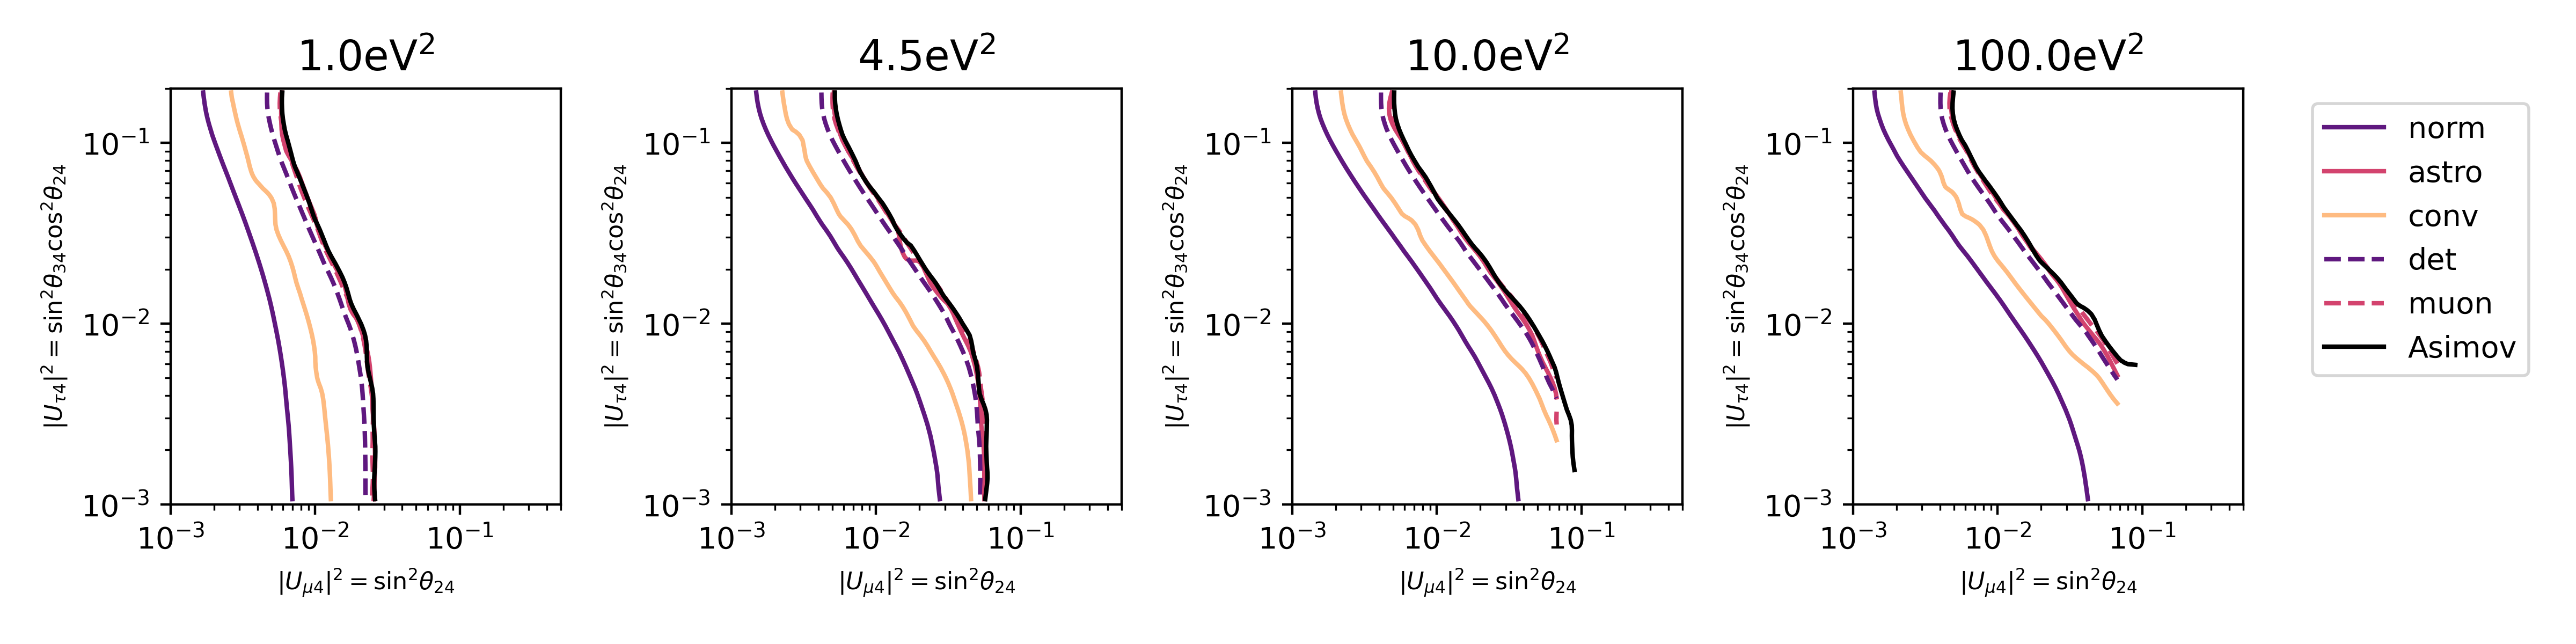
\includegraphics[width=0.90\linewidth]{figures/systematic_impact_joint.png}
    \caption{The sensitivity contours for fixing each bundle of nuisance parameters. Contours are shown at 90\% CL and 3DOF for various mass-squared splittings; from left to right: 1.0eV$^{2}$, 4.5eV$^{2}$, 10.0eV$^{2}$, and 100.0eV$^{2}$.}\label{fig:impact}
\end{figure}

\subsection{Signal Inject-Recover}

Various points were chosen along the Asimov 90\% CL thresholds to test the fitting framework's ability to recover constraints of sterile-neutrino signal-like measurements. 
Two each were chosen along the contours at 1.0, 4.5, and 10 eV$^{2}$; one more was chosen at 100 eV$^{2}$. 
Additionally, three more points were chosen off-grid at various points.
Of those three, one was selected as the recovered best-fit point from the 8-year track analysis. 
Each of these points are listed in Table~\ref{table:injected_signals}.
Then, we ran a full fit-scan on an Asimov realization generated for each of these simulated signals. 
Injected values are recovered in all cases where a signal is injected at a grid-point. 
For the cases where a signal is injected near a grid point, the best fit is sufficiently close.

\begin{table}
    \centering
    \rowcolors{2}{gray!25}{white}
    \begin{tabular}{c | cccc}\rowcolor{blue!25}
            Realization Name & $\theta_{14}$ [rad] & $\theta_{24}$ [rad] & $\theta_{34}$ [rad] & $\Delta m_{41}^{2}$ [eV$^{2}$] \\
            RealIR\_0& 0.0  & 0.08192326 & 0.3206565 & 1.0 \\
            RealIR\_1& 0.0  & 0.1473121 & 0.077387 & 1.0\\
            RealIR\_2& 0.0  & 0.2295065 & 0.07861259 & 4.5\\
            RealIR\_3& 0.0  & 0.08192326 & 0.3206565 & 4.5\\
            RealIR\_4& 0.0  & 0.3096057 & 0.2337925 & 10.0\\
            RealIR\_5& 0.0  & 0.0948438 & 0.223506 & 10.0\\
            RealIR\_6& 0.0  & 0.1473121 & 0.1317024 & 100\\
            RealIR\_7$^{\dag}$ & 0.0  & 0.02 & 0.02 & 2.0\\
            RealIR\_8$^{\dag}$ & 0.0  & 0.08 & 0.003 & 7.0\\
            RealIR\_9$^{\dag}$ & 0.0  & 0.1609 & 0.0 & 4.5
    \end{tabular}
    \caption{Sterile neutrino mixing angles at which Asimov realizations were generated. Entries marked with $\dag$ were generated off of the grid used for fit scans.}\label{table:injected_signals}
\end{table}

\begin{figure}
    \centering
    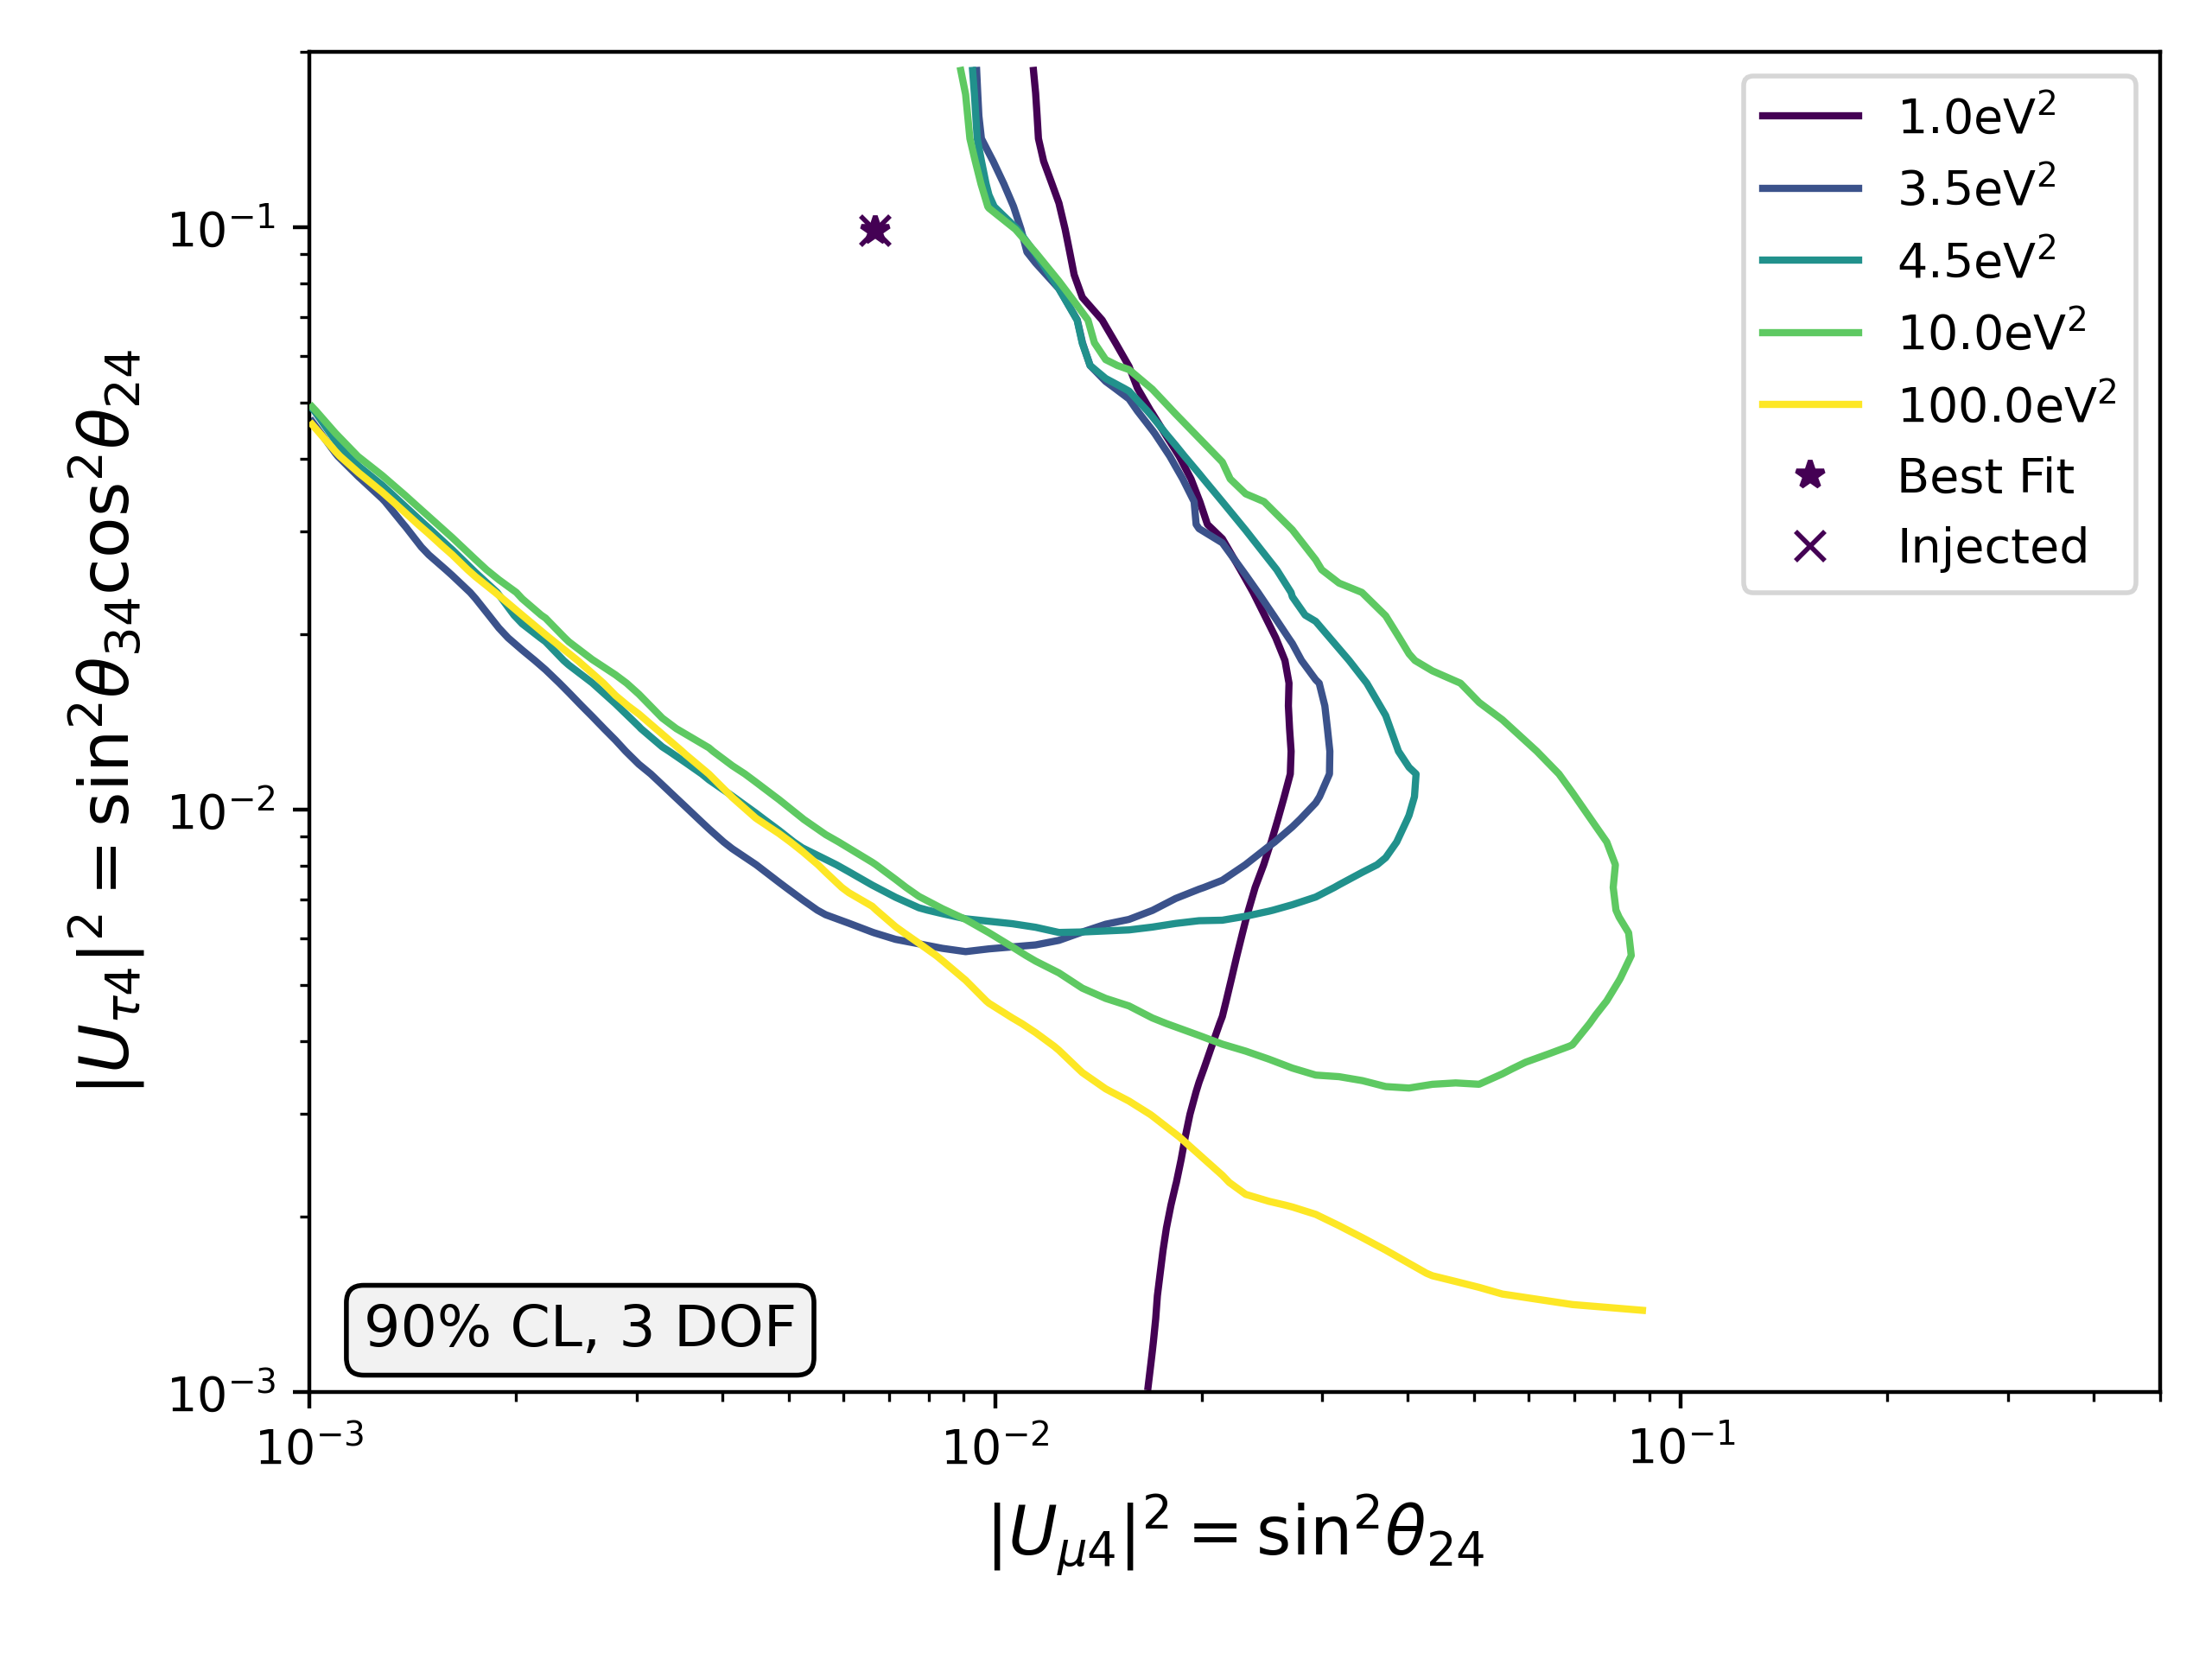
\includegraphics[width=0.45\linewidth]{figures/inject_recover_RealIR_0_sterile_1_cl0.9_dof3.png}%
    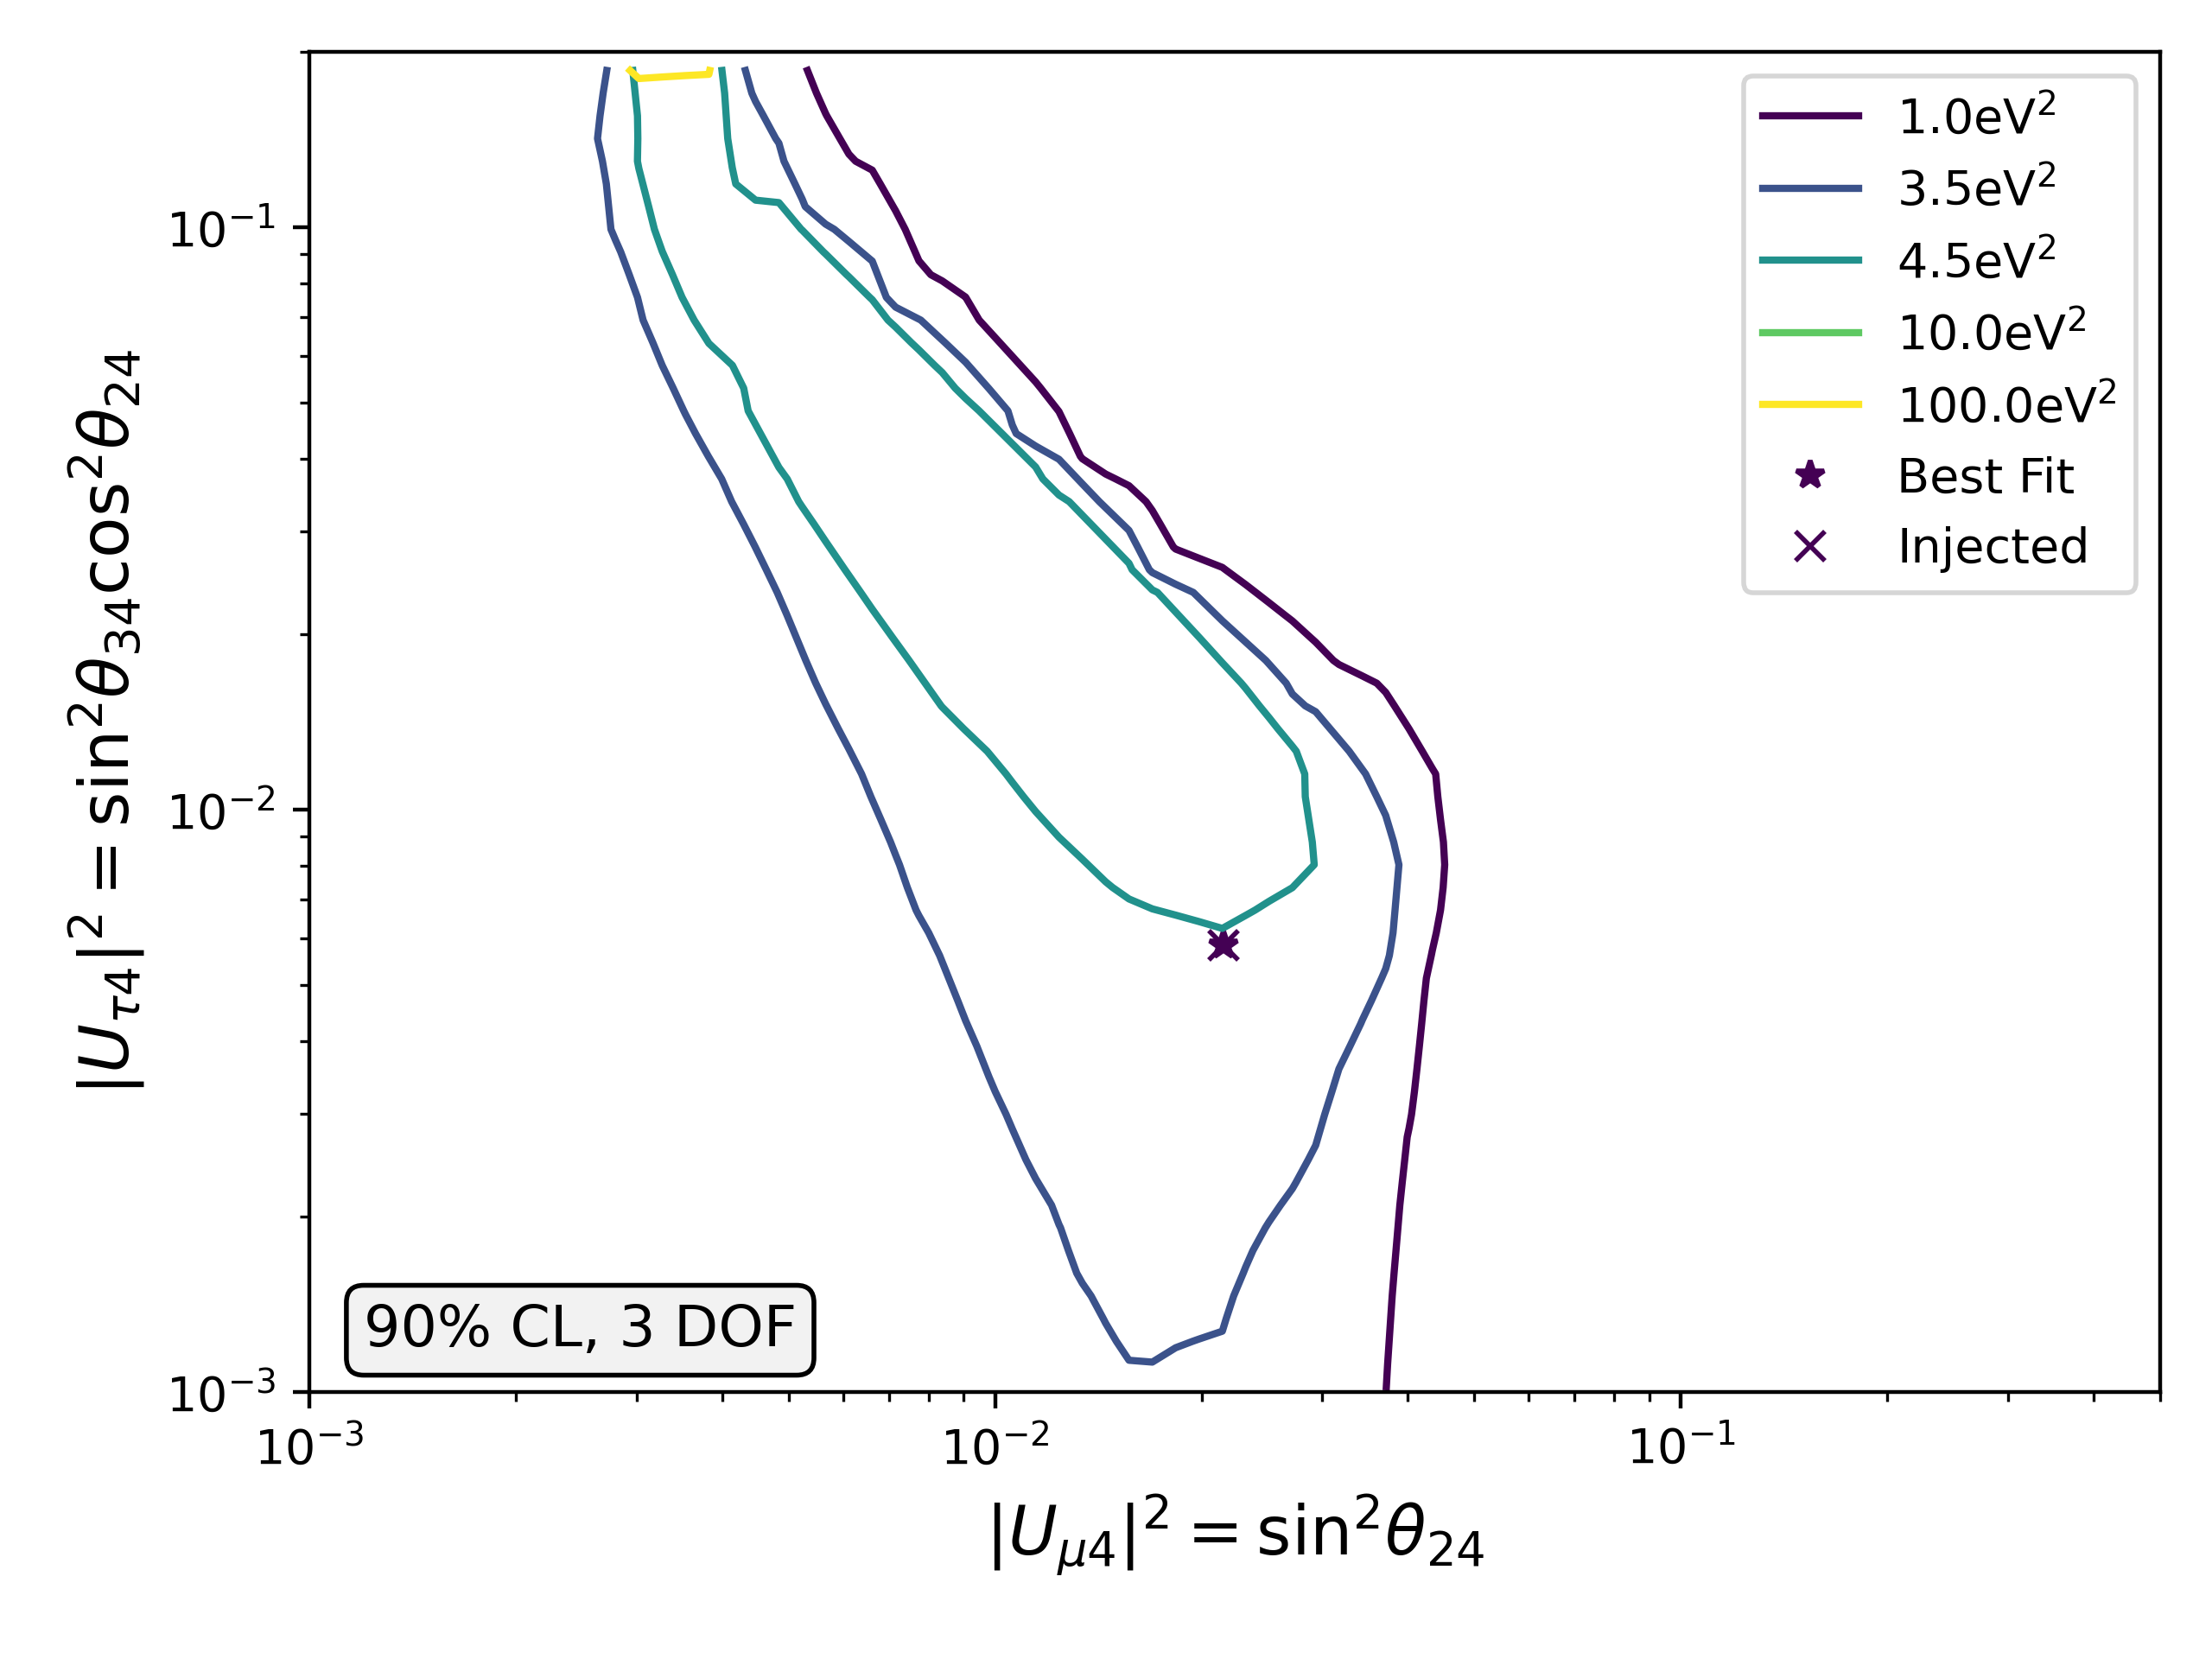
\includegraphics[width=0.45\linewidth]{figures/inject_recover_RealIR_1_sterile_1_cl0.9_dof3.png}
    \caption{To be added later}
\end{figure}

\begin{figure}
    \centering
    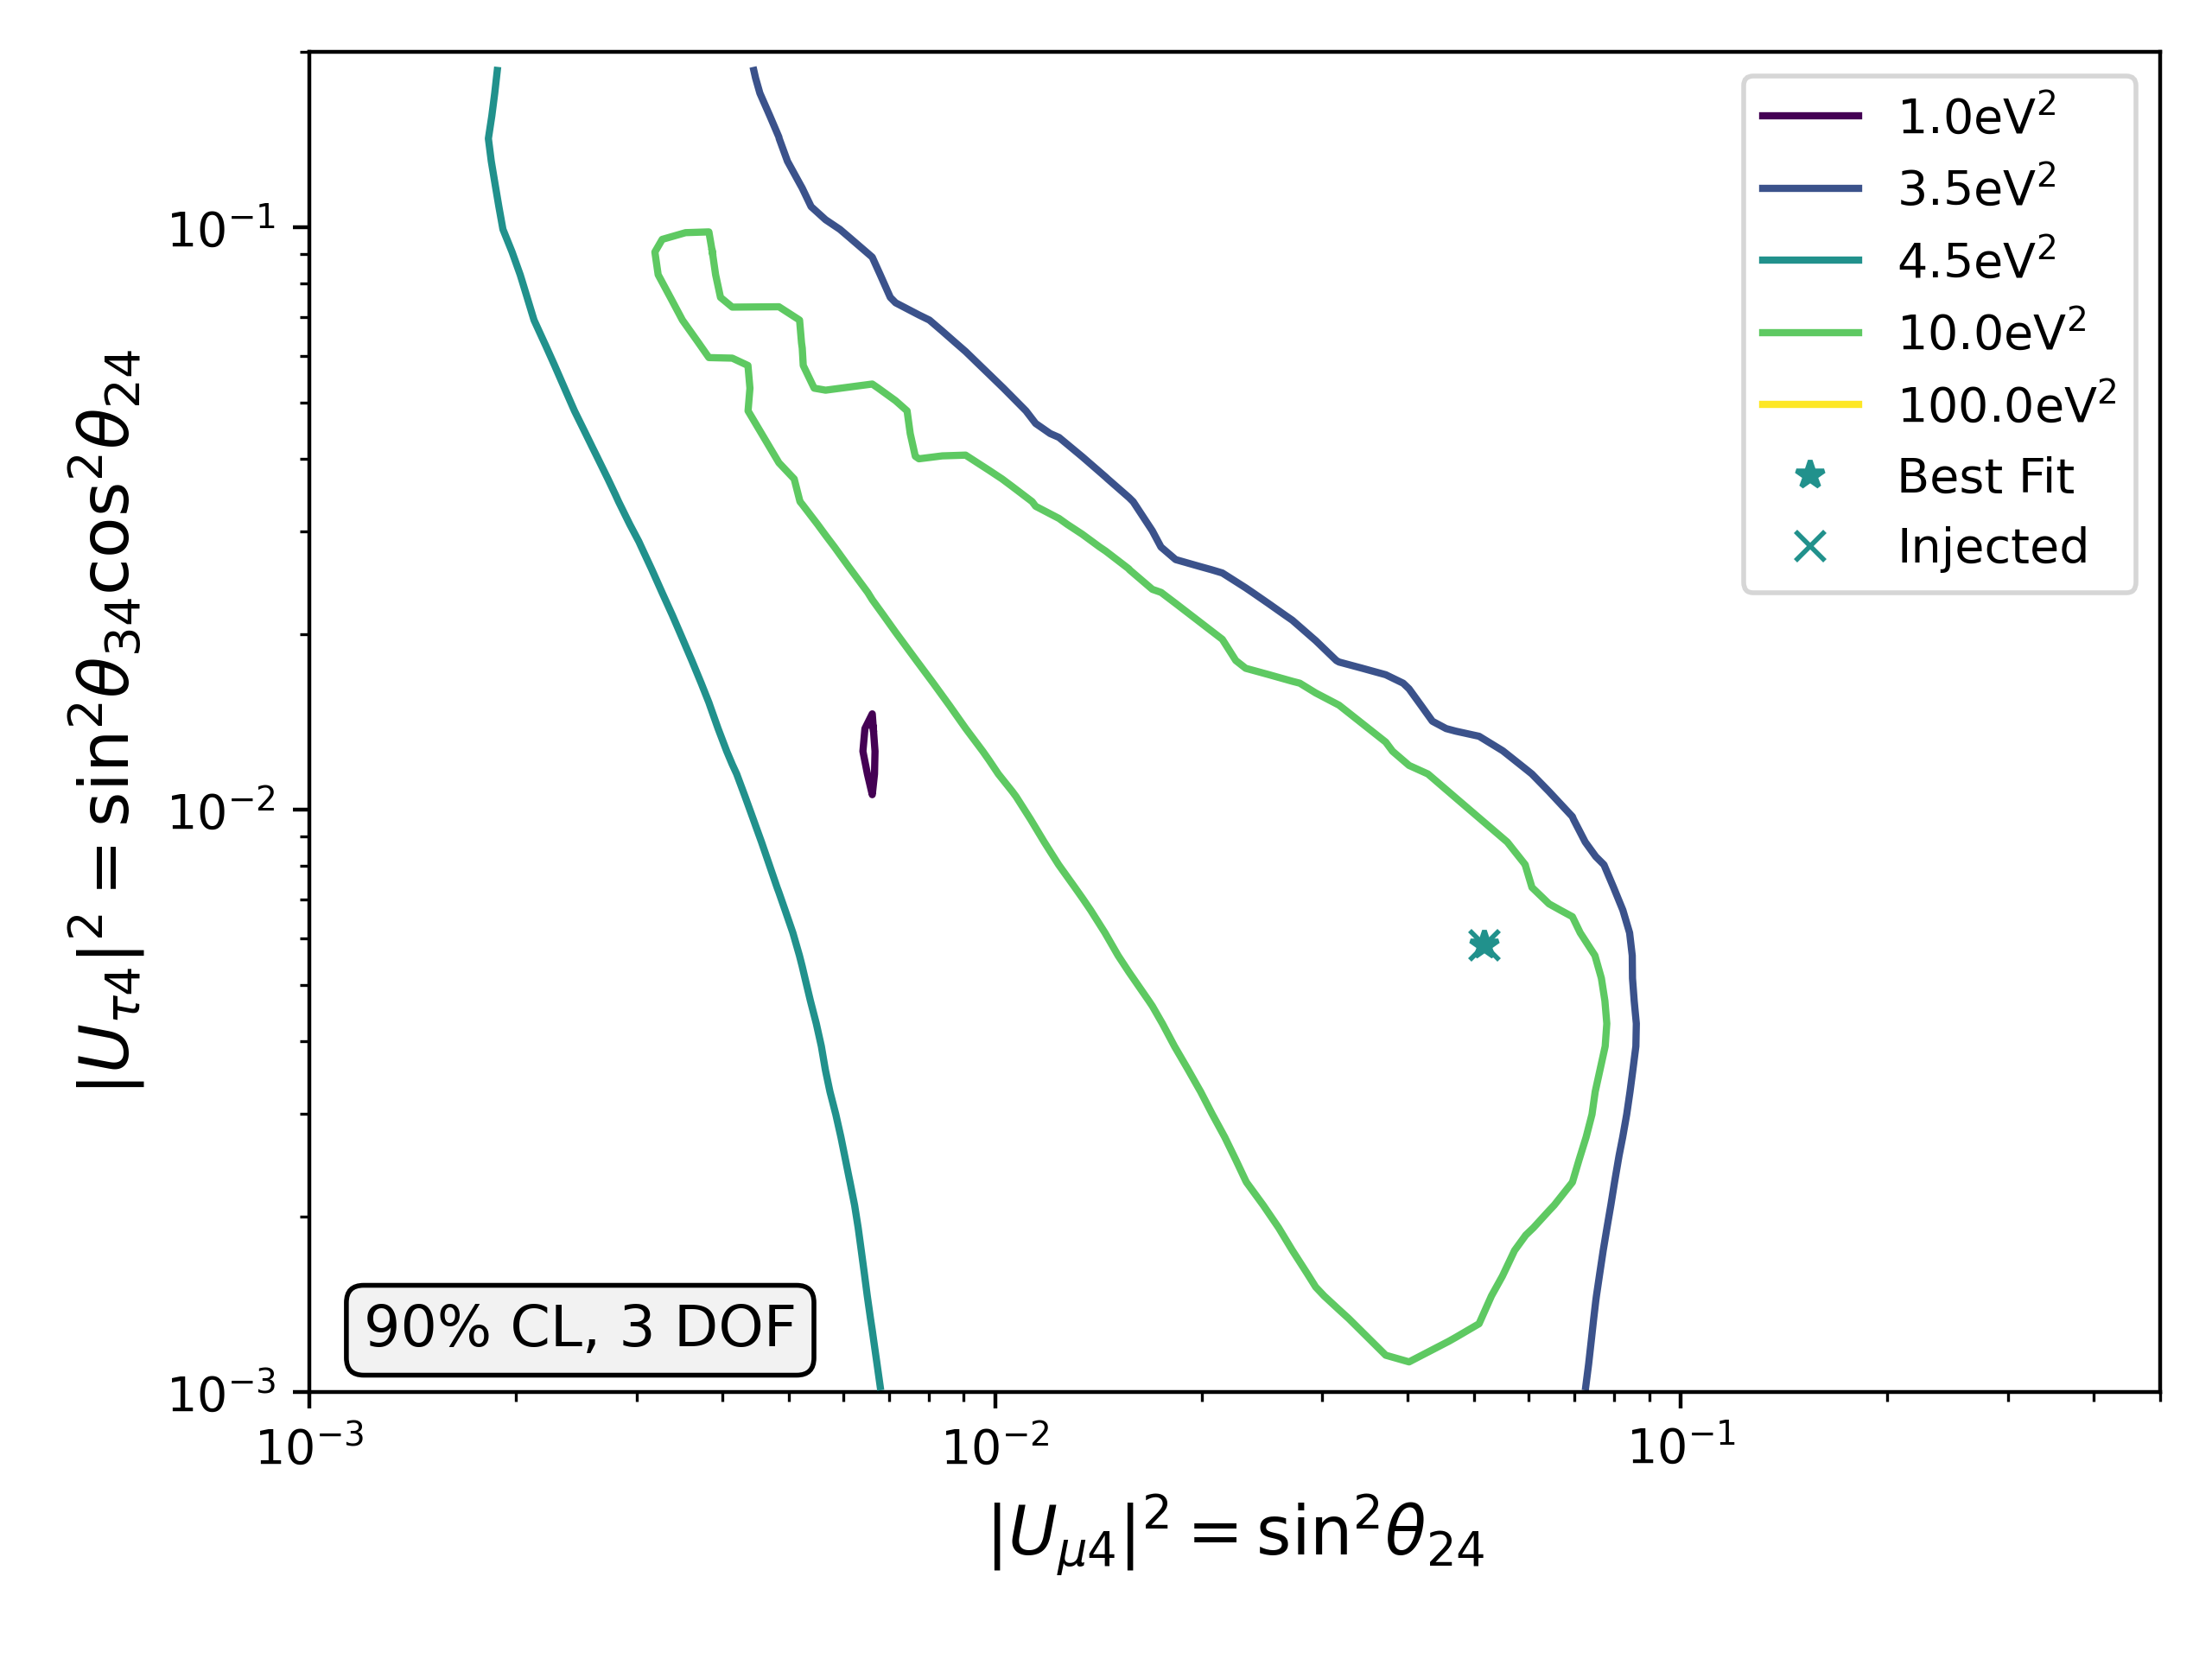
\includegraphics[width=0.45\linewidth]{figures/inject_recover_RealIR_2_sterile_4_cl0.9_dof3.png}%
    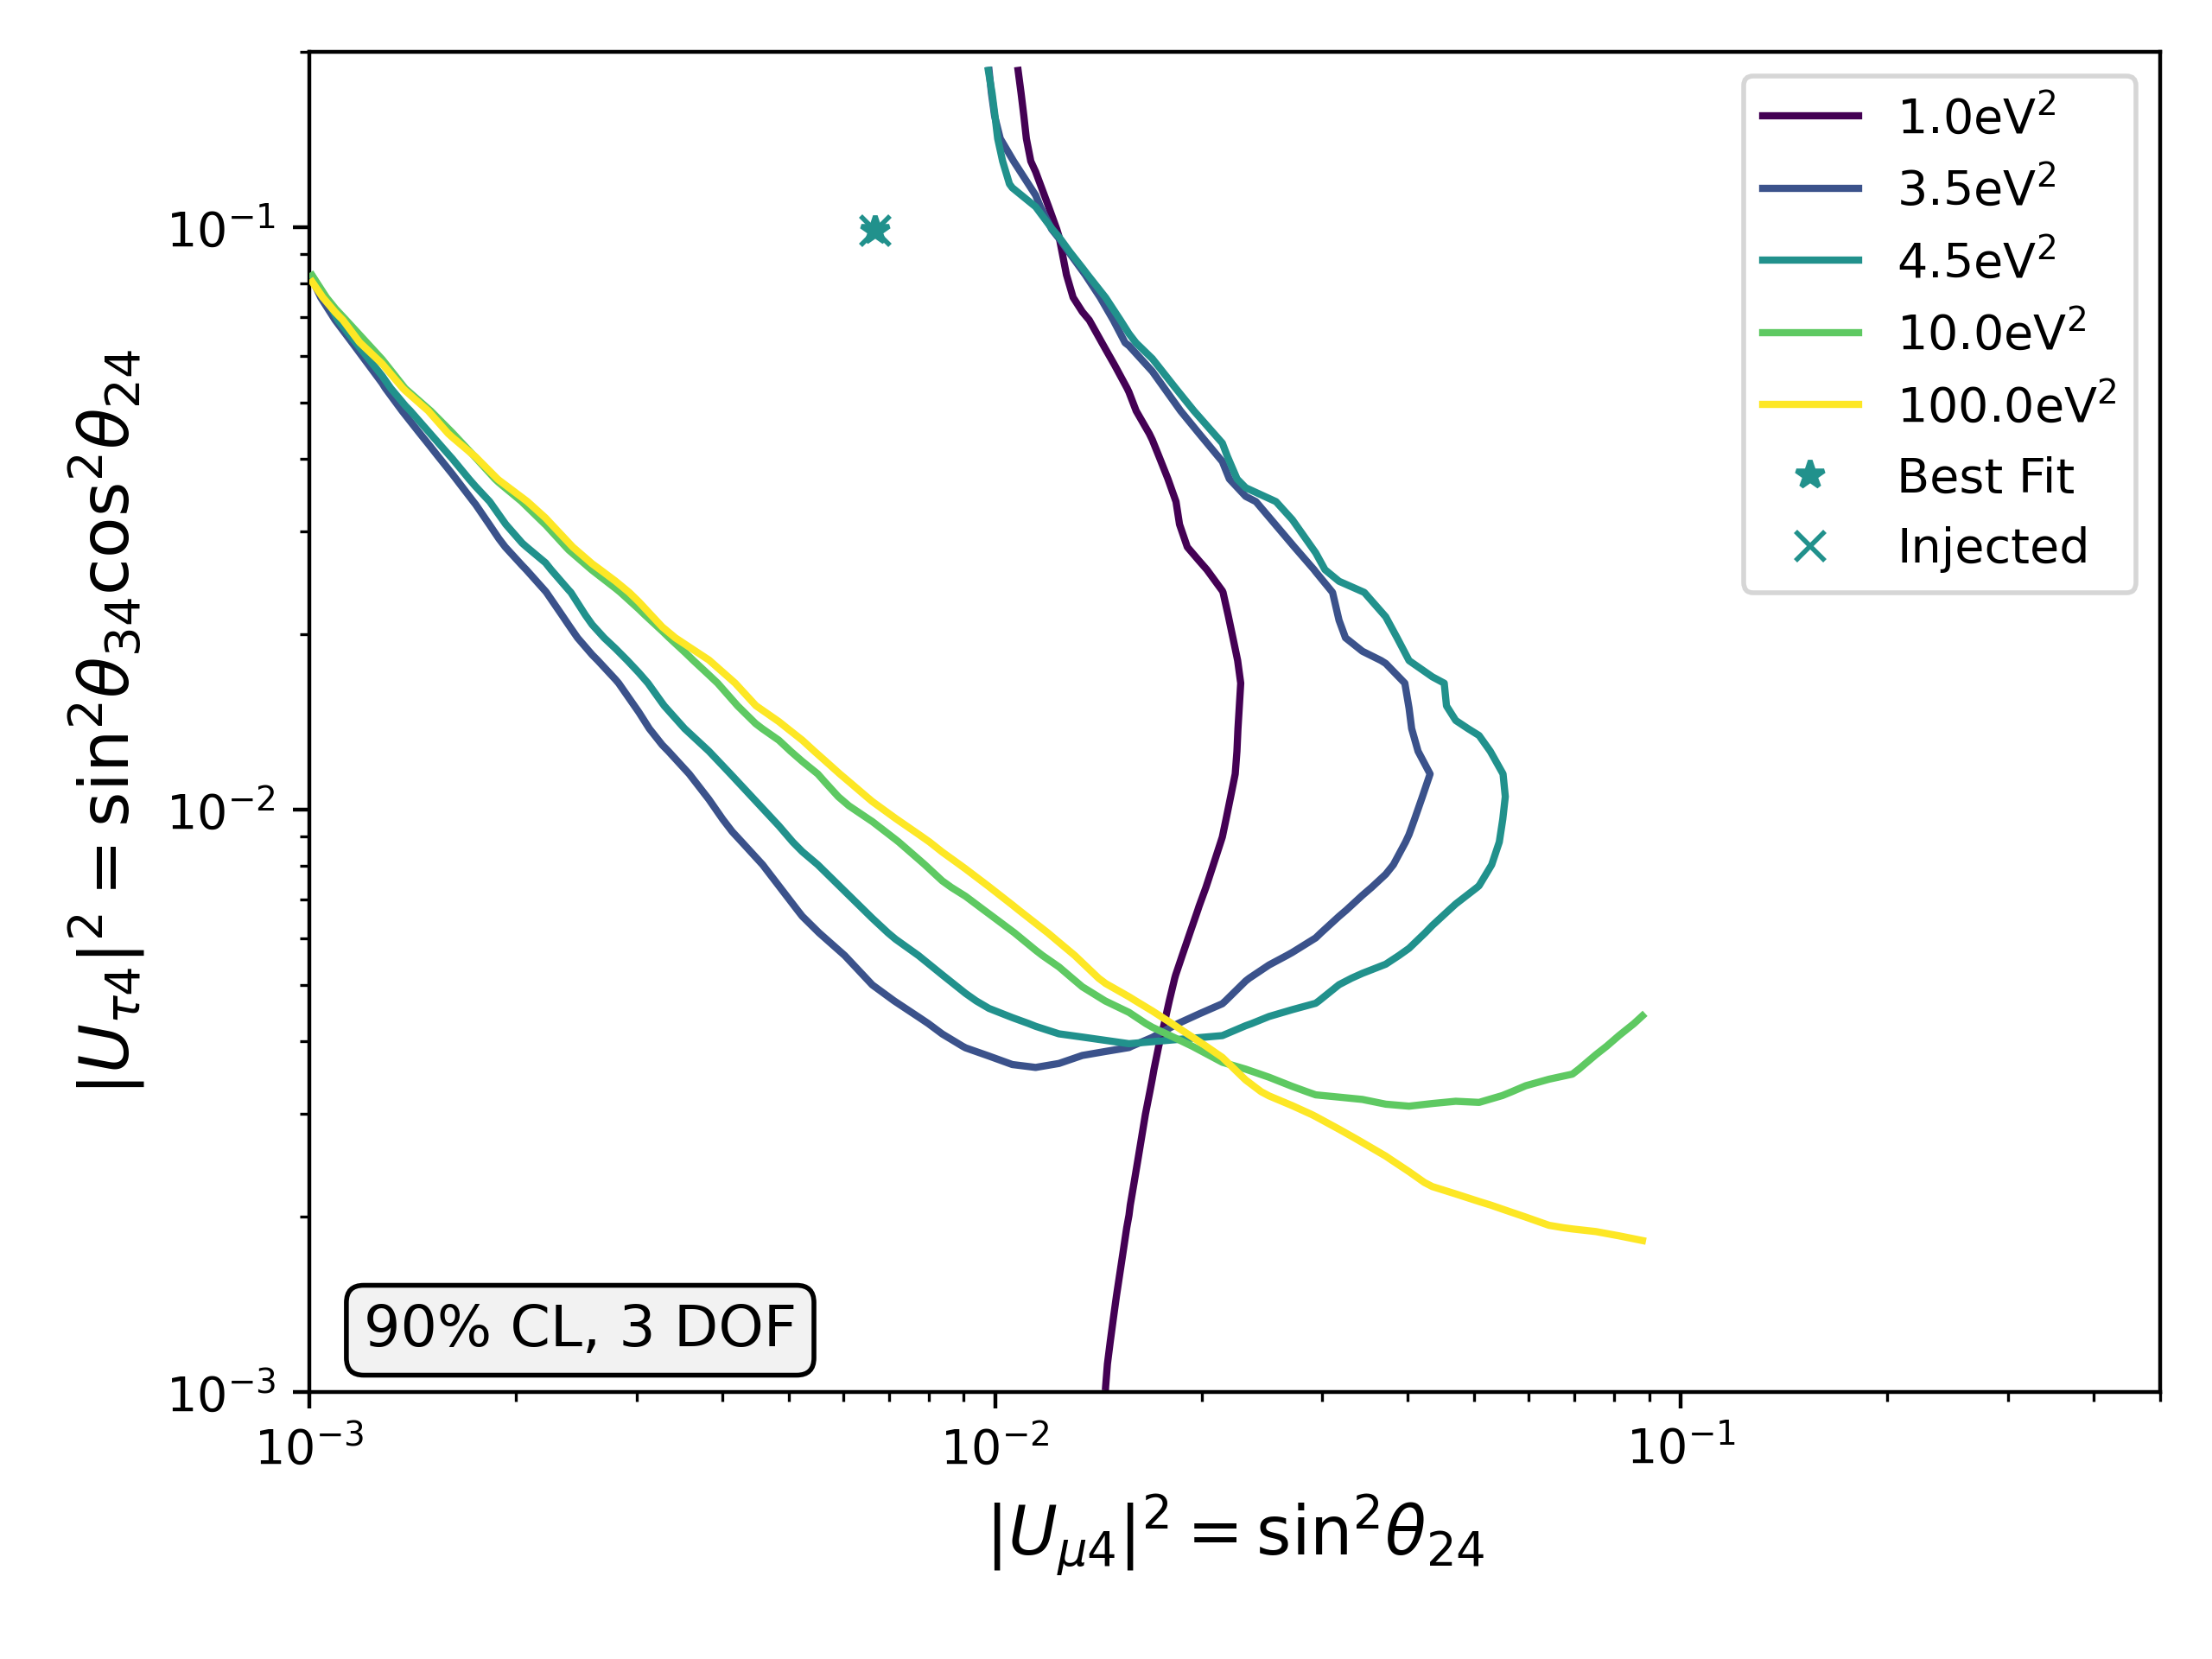
\includegraphics[width=0.45\linewidth]{figures/inject_recover_RealIR_3_sterile_4_cl0.9_dof3.png}
    \caption{To be added later}
\end{figure}


\begin{figure}
    \centering
    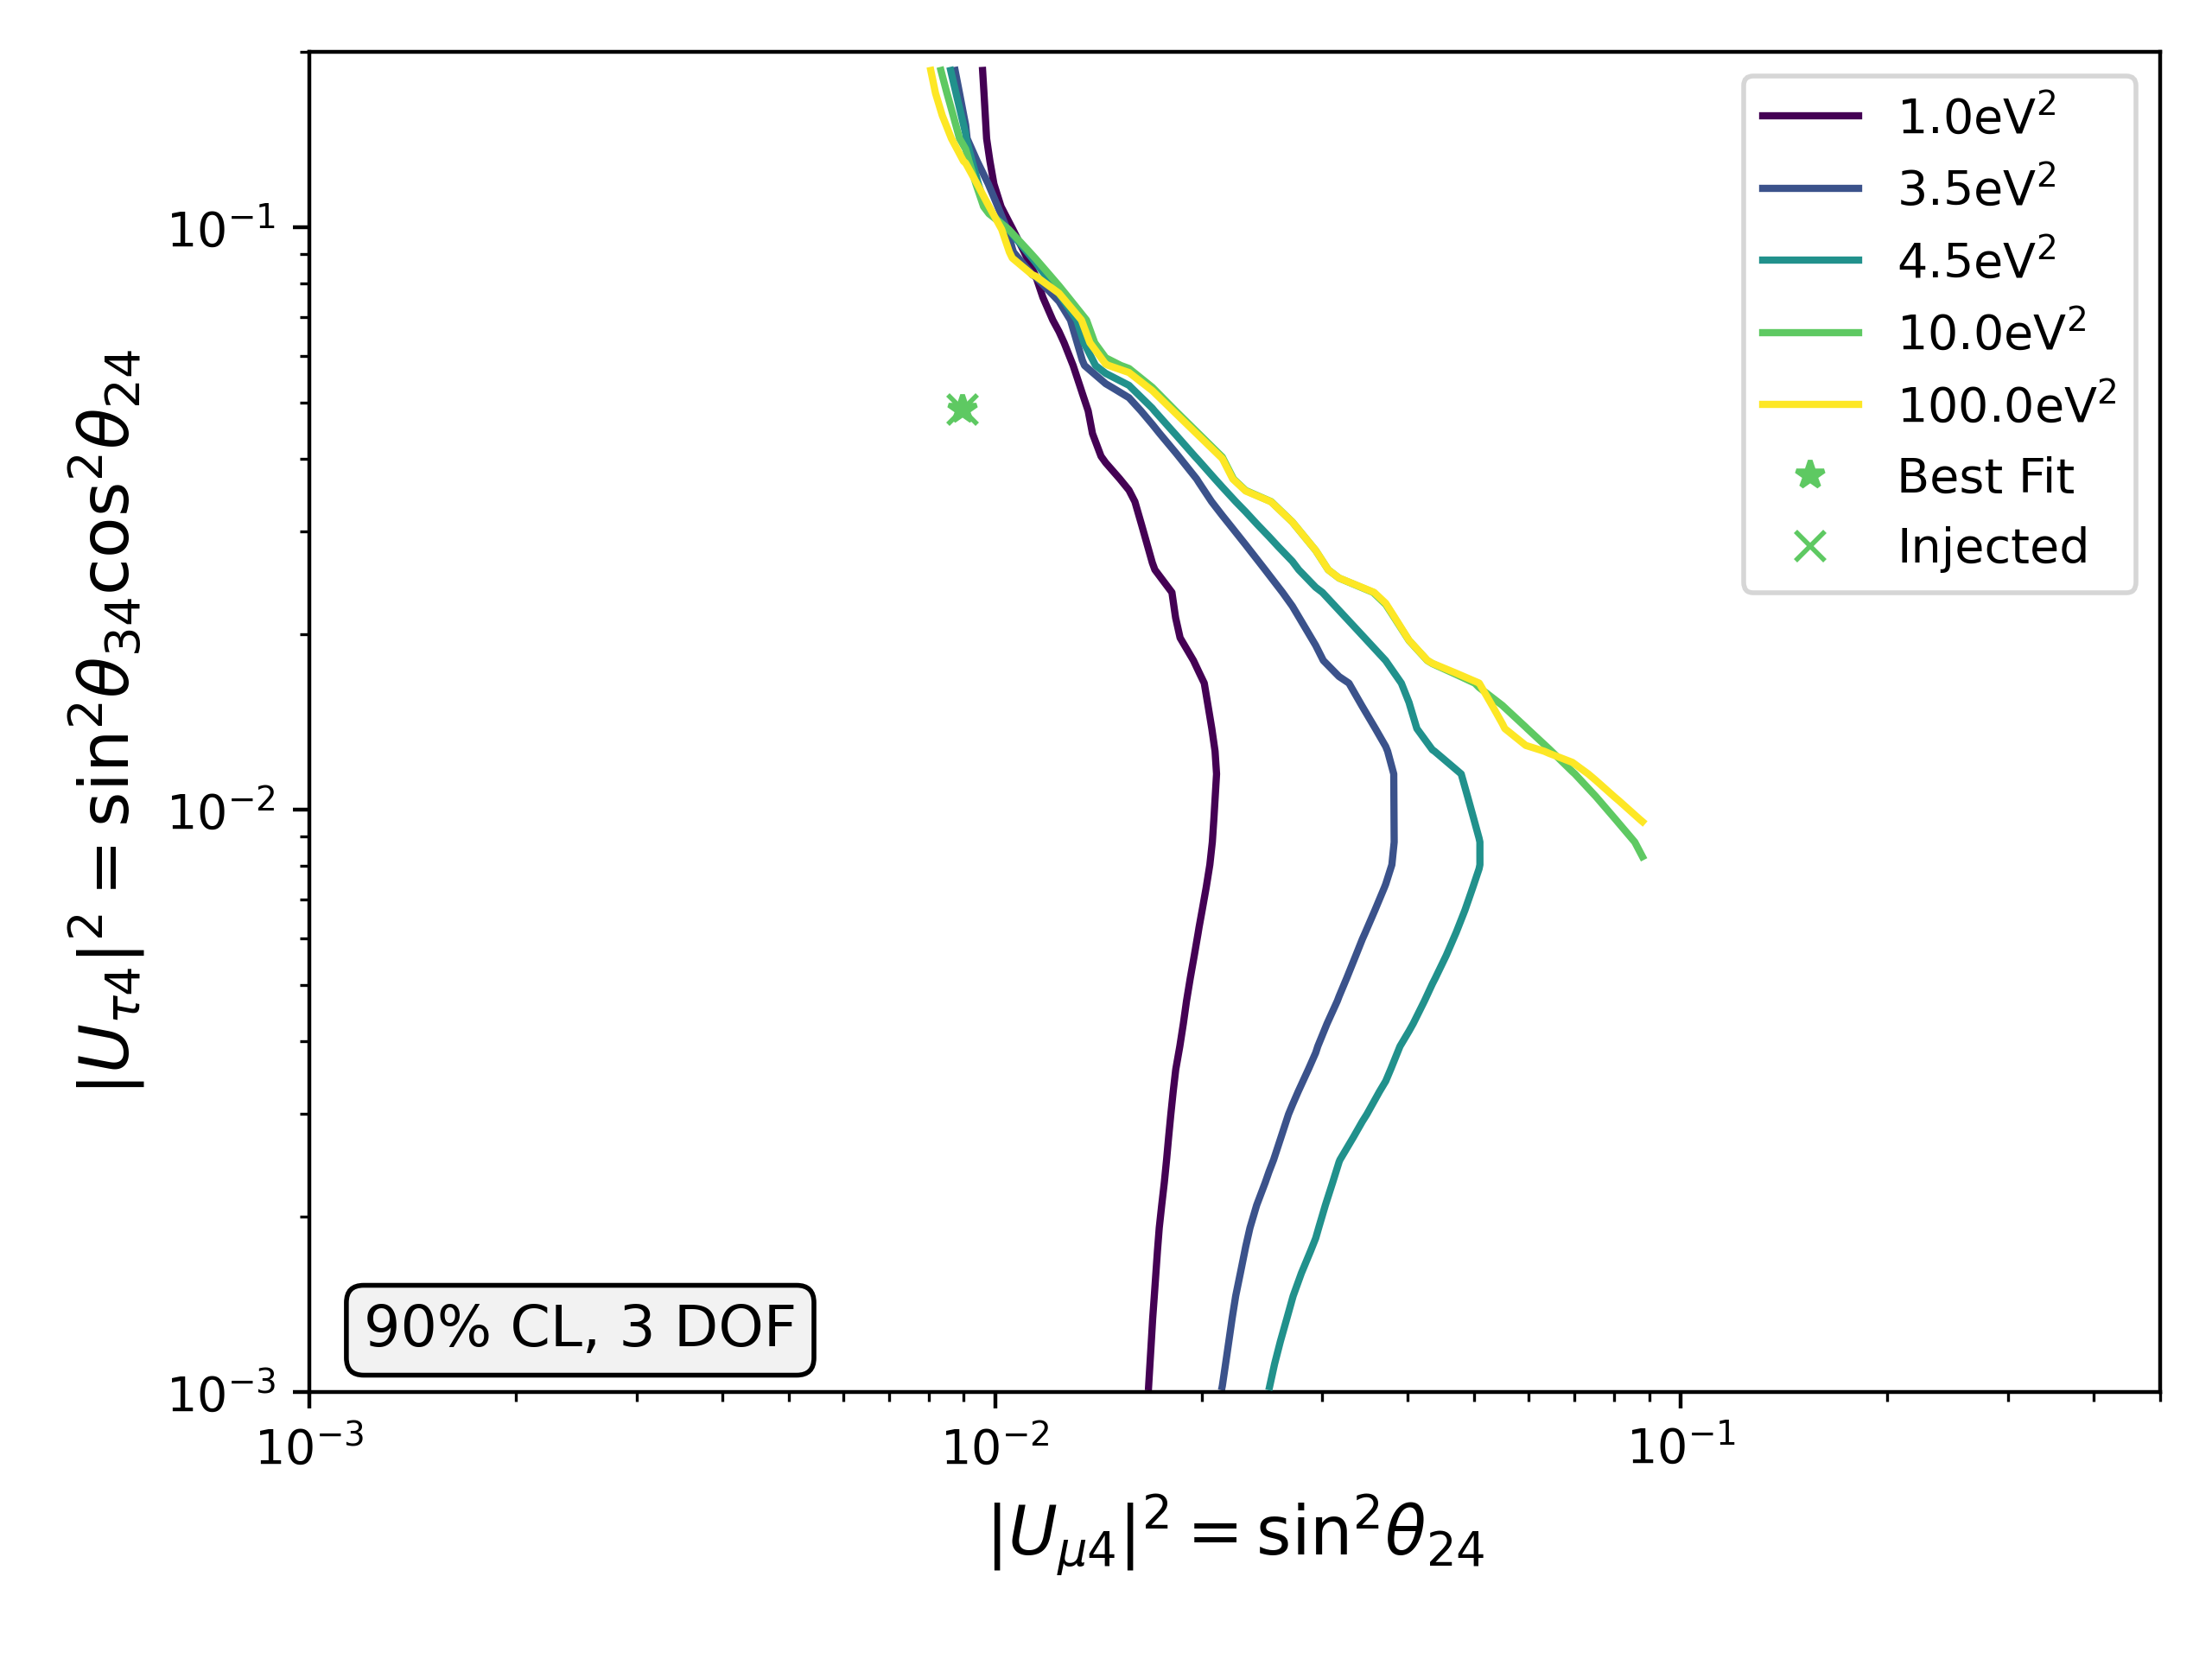
\includegraphics[width=0.45\linewidth]{figures/inject_recover_RealIR_5_sterile_1_cl0.9_dof3.png}%
    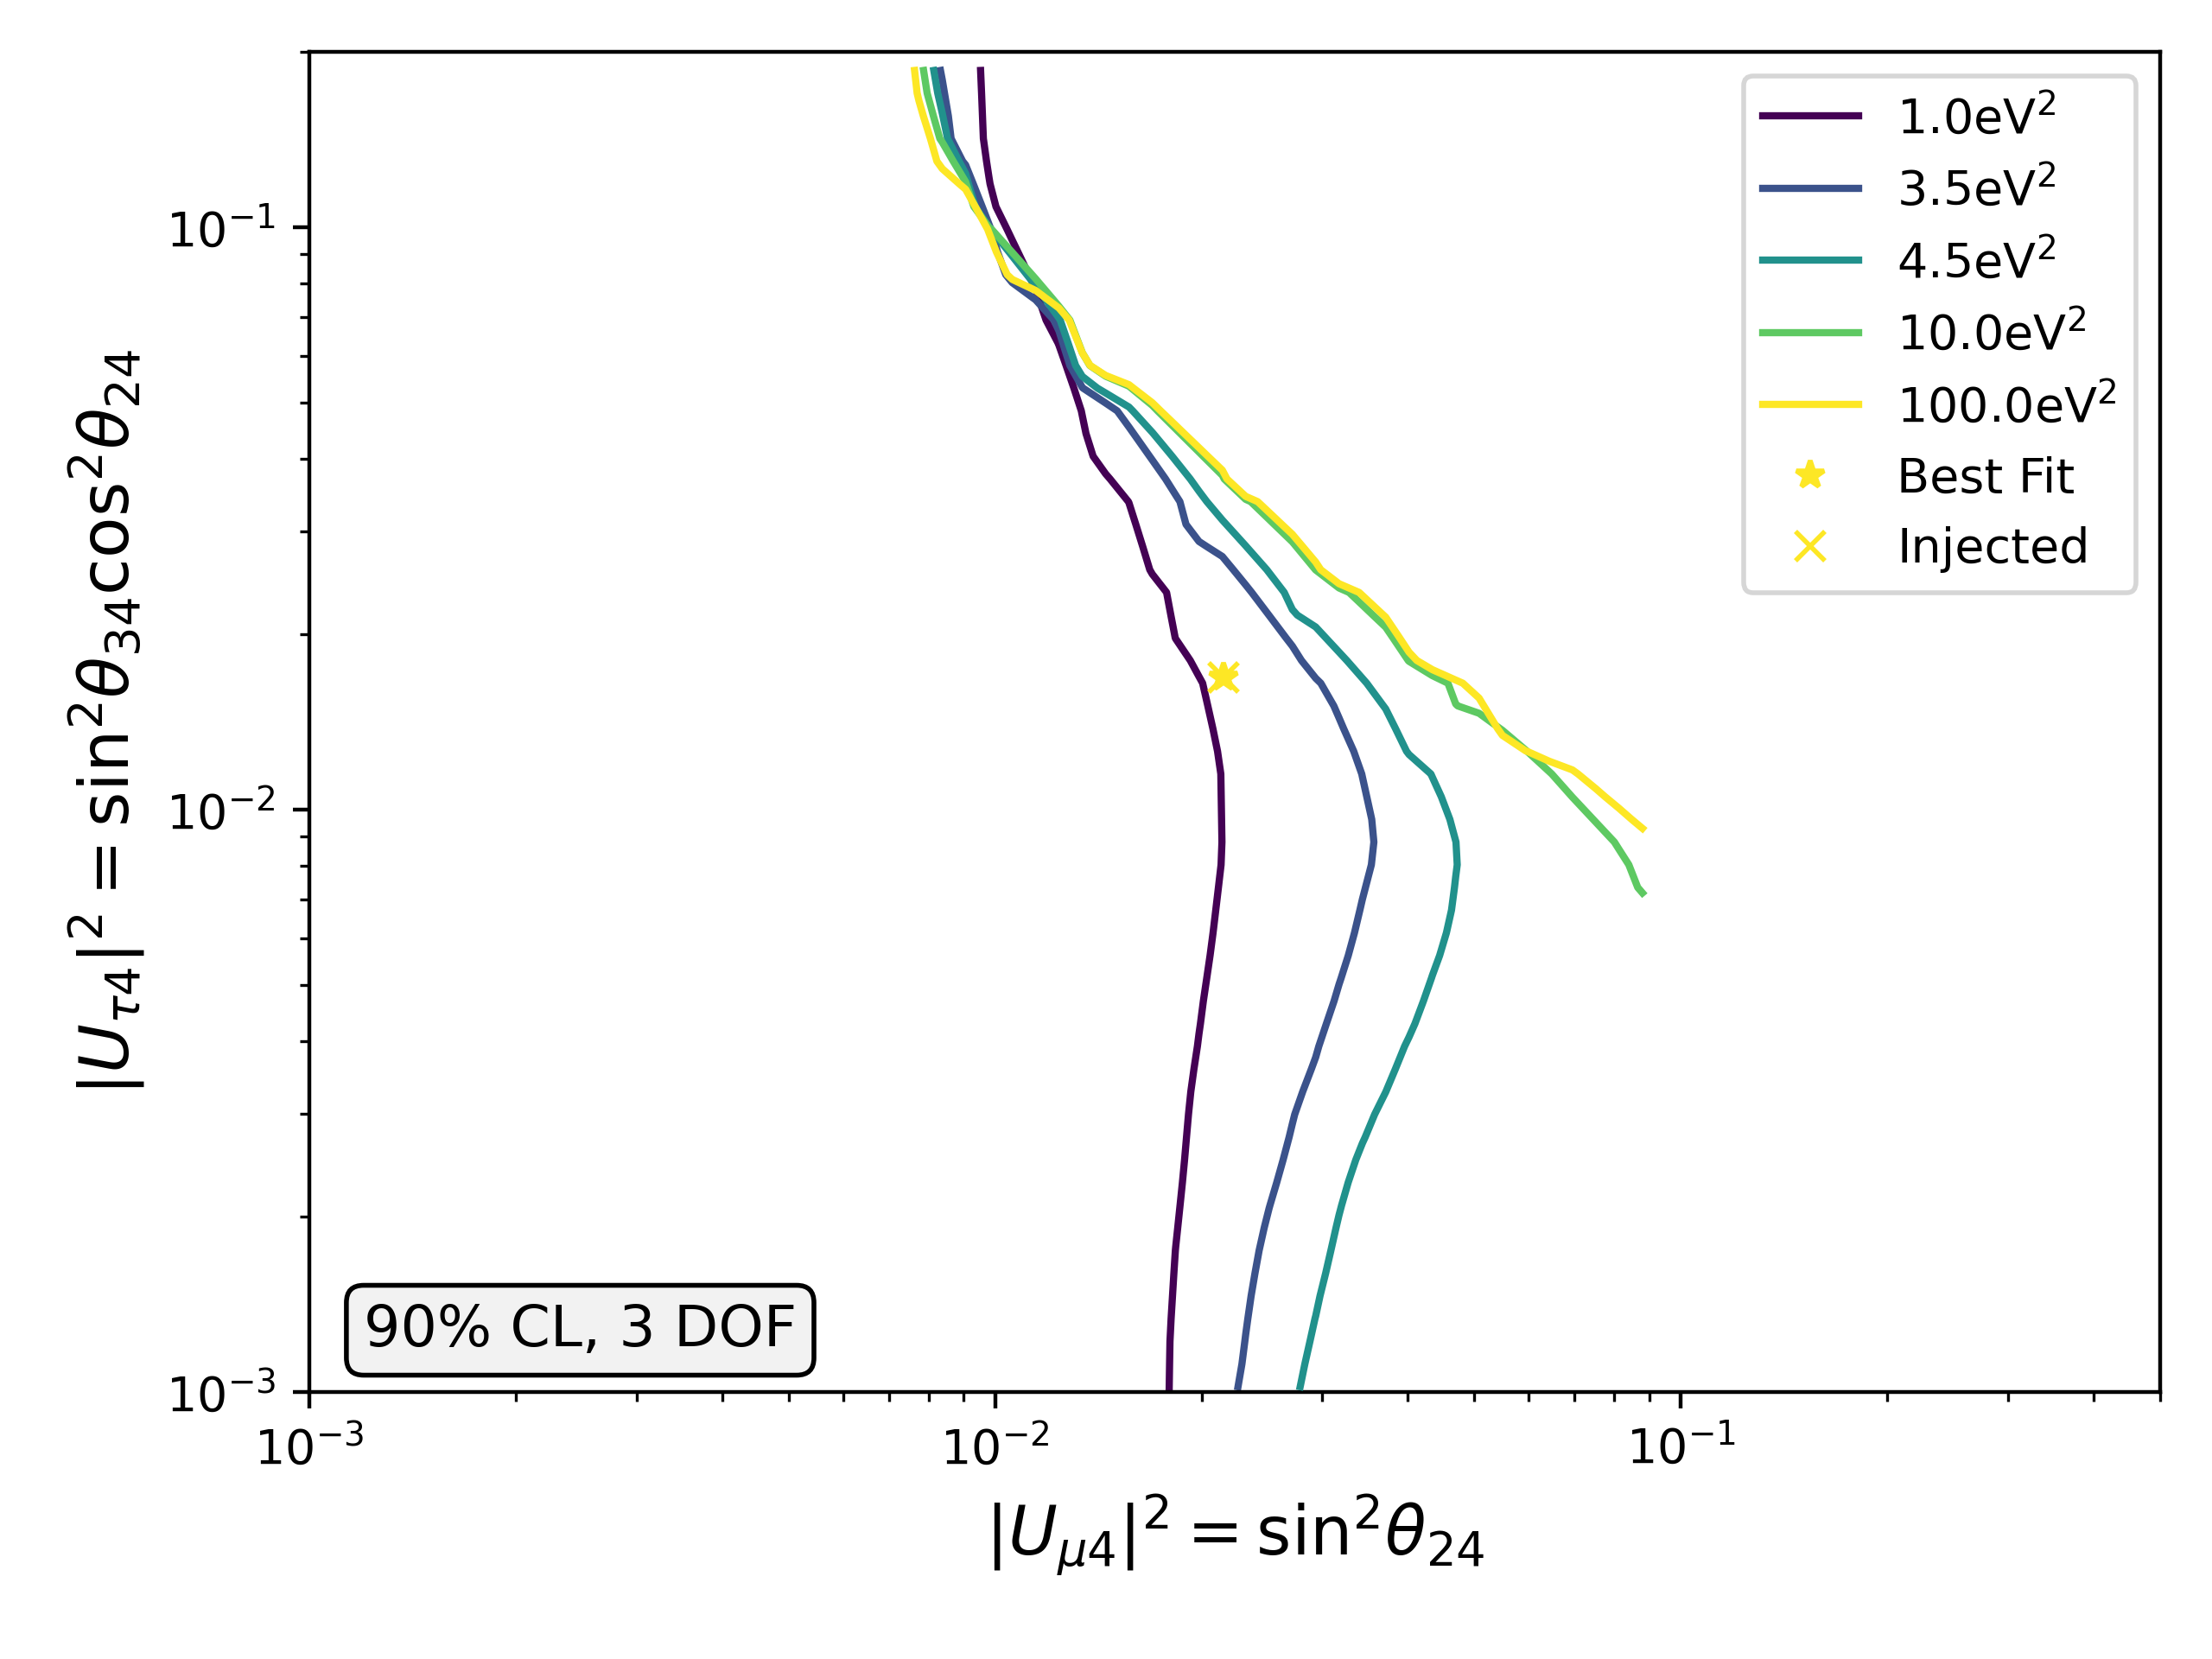
\includegraphics[width=0.45\linewidth]{figures/inject_recover_RealIR_6_sterile_1_cl0.9_dof3.png}
    \caption{To be added later}
\end{figure}

\begin{figure}
    \centering
    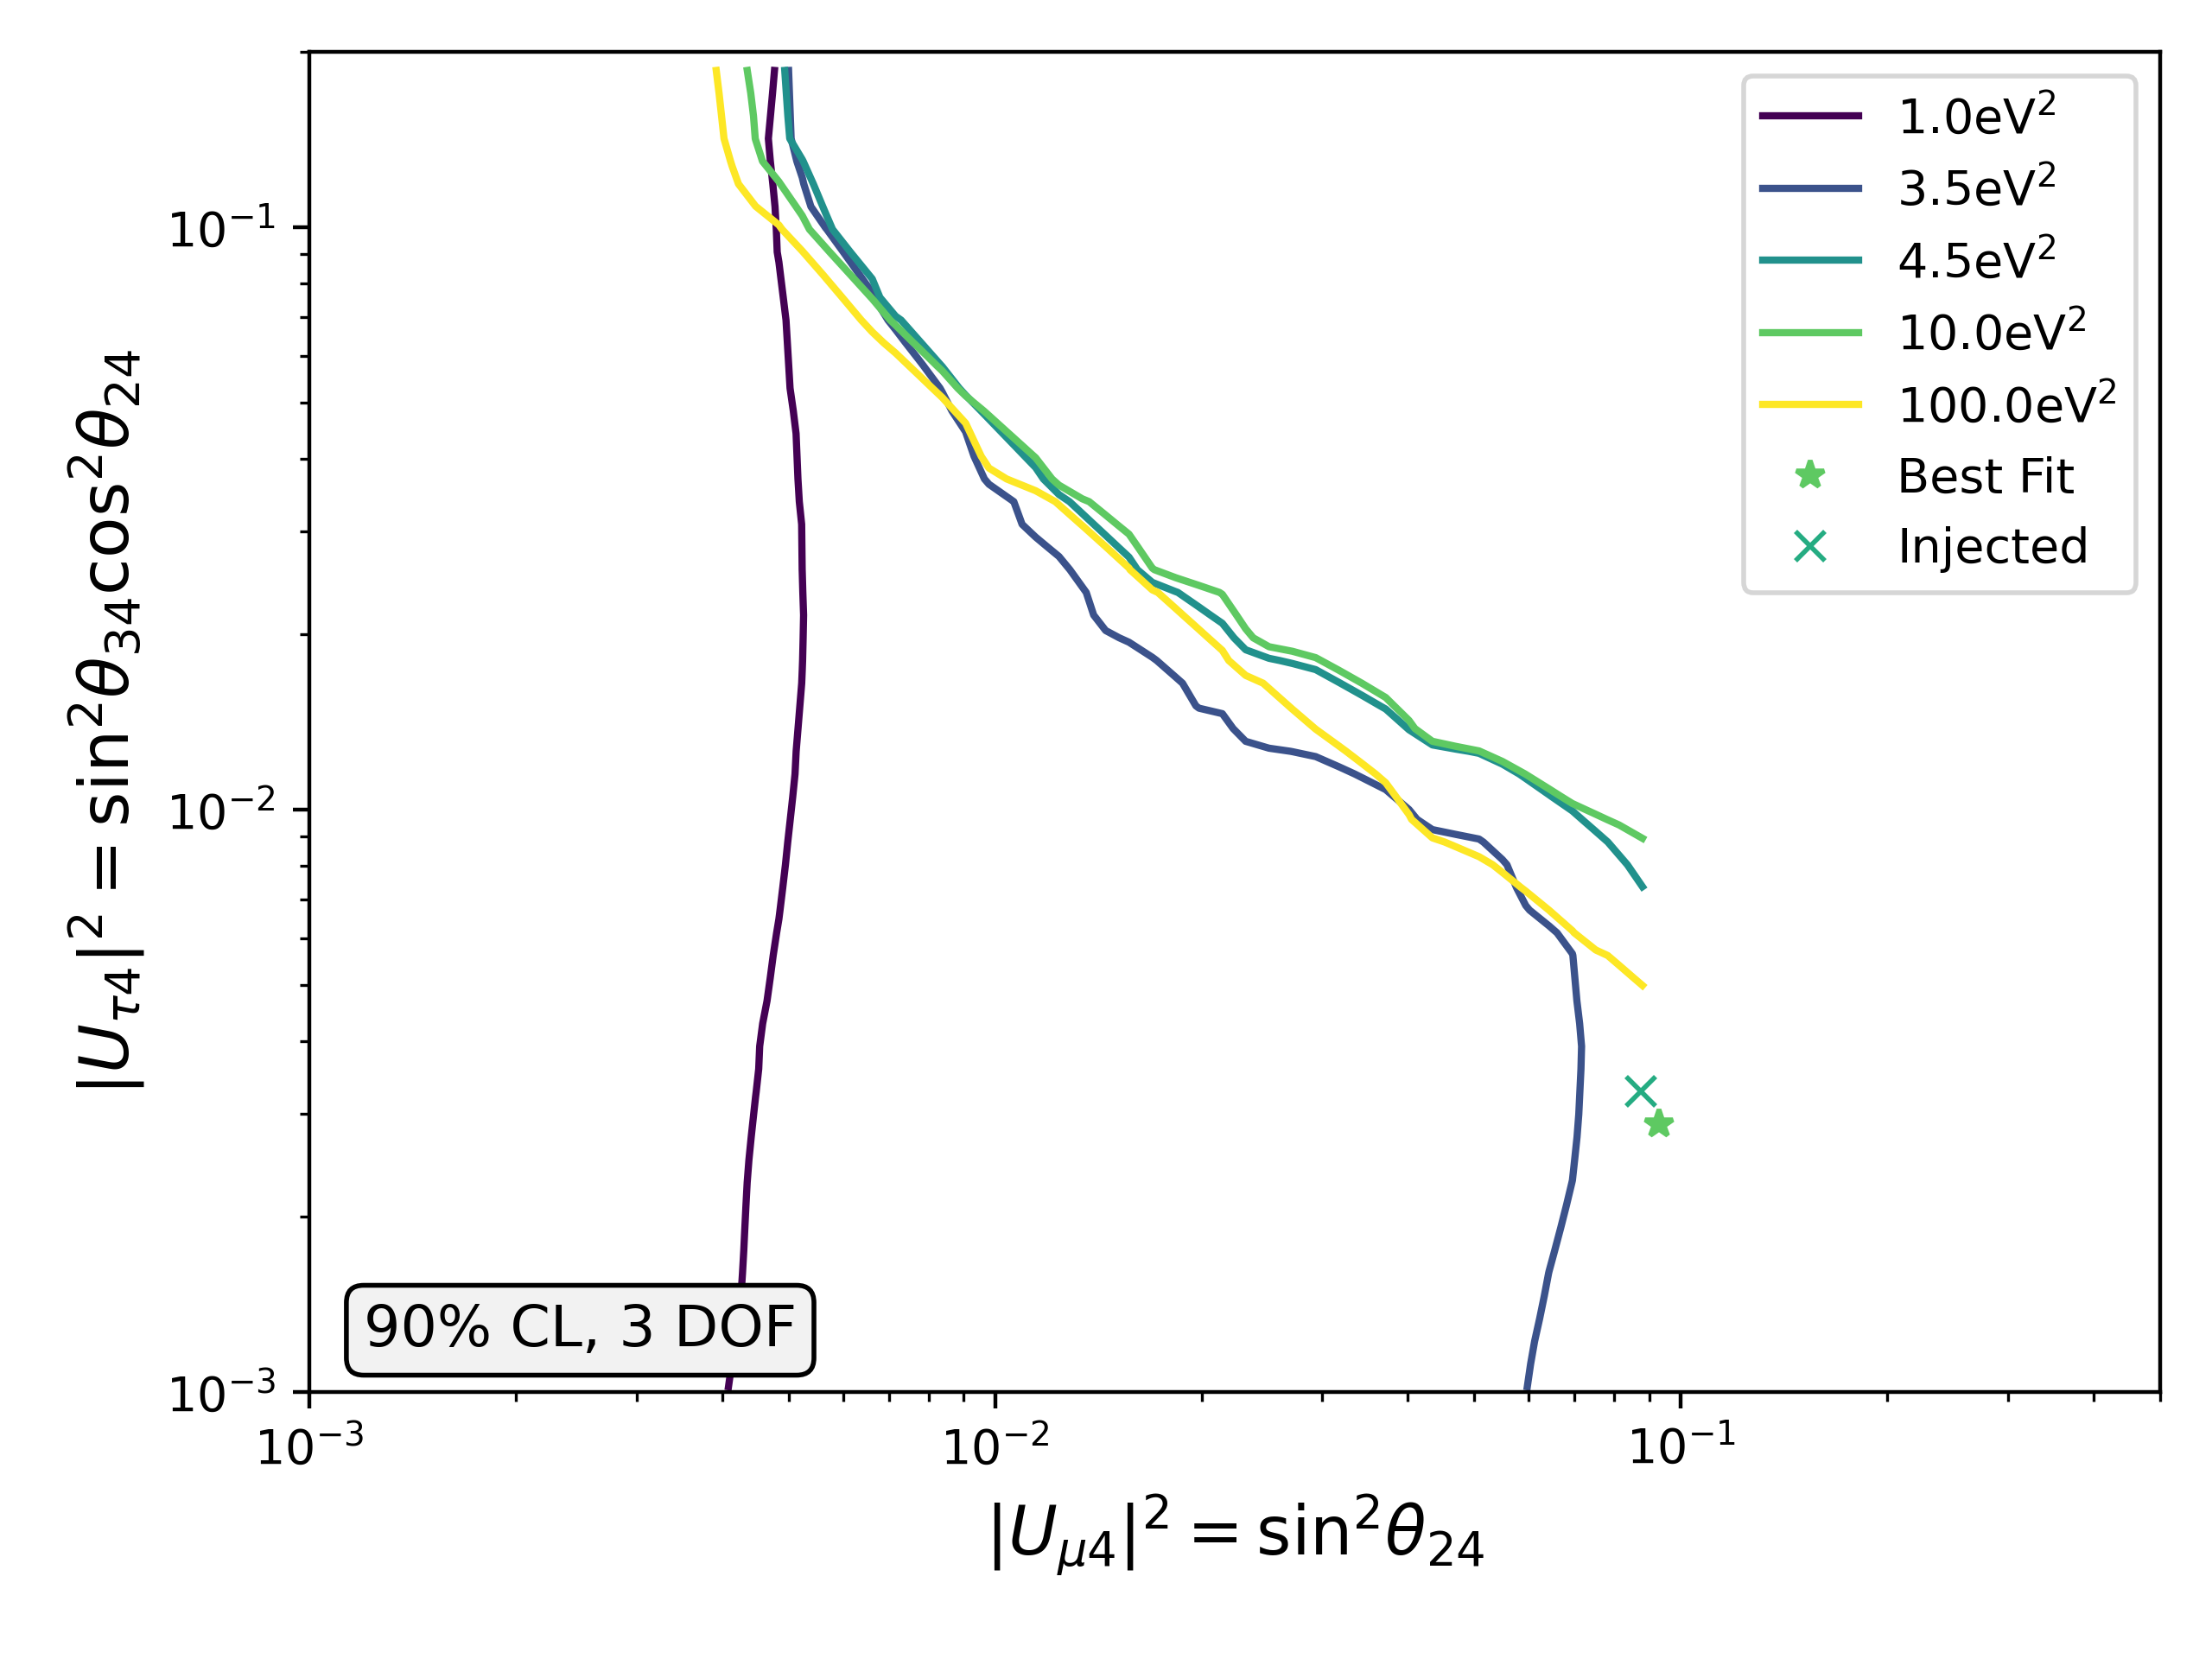
\includegraphics[width=0.45\linewidth]{figures/inject_recover_RealIR_8_sterile_7_cl0.9_dof3.png}%
    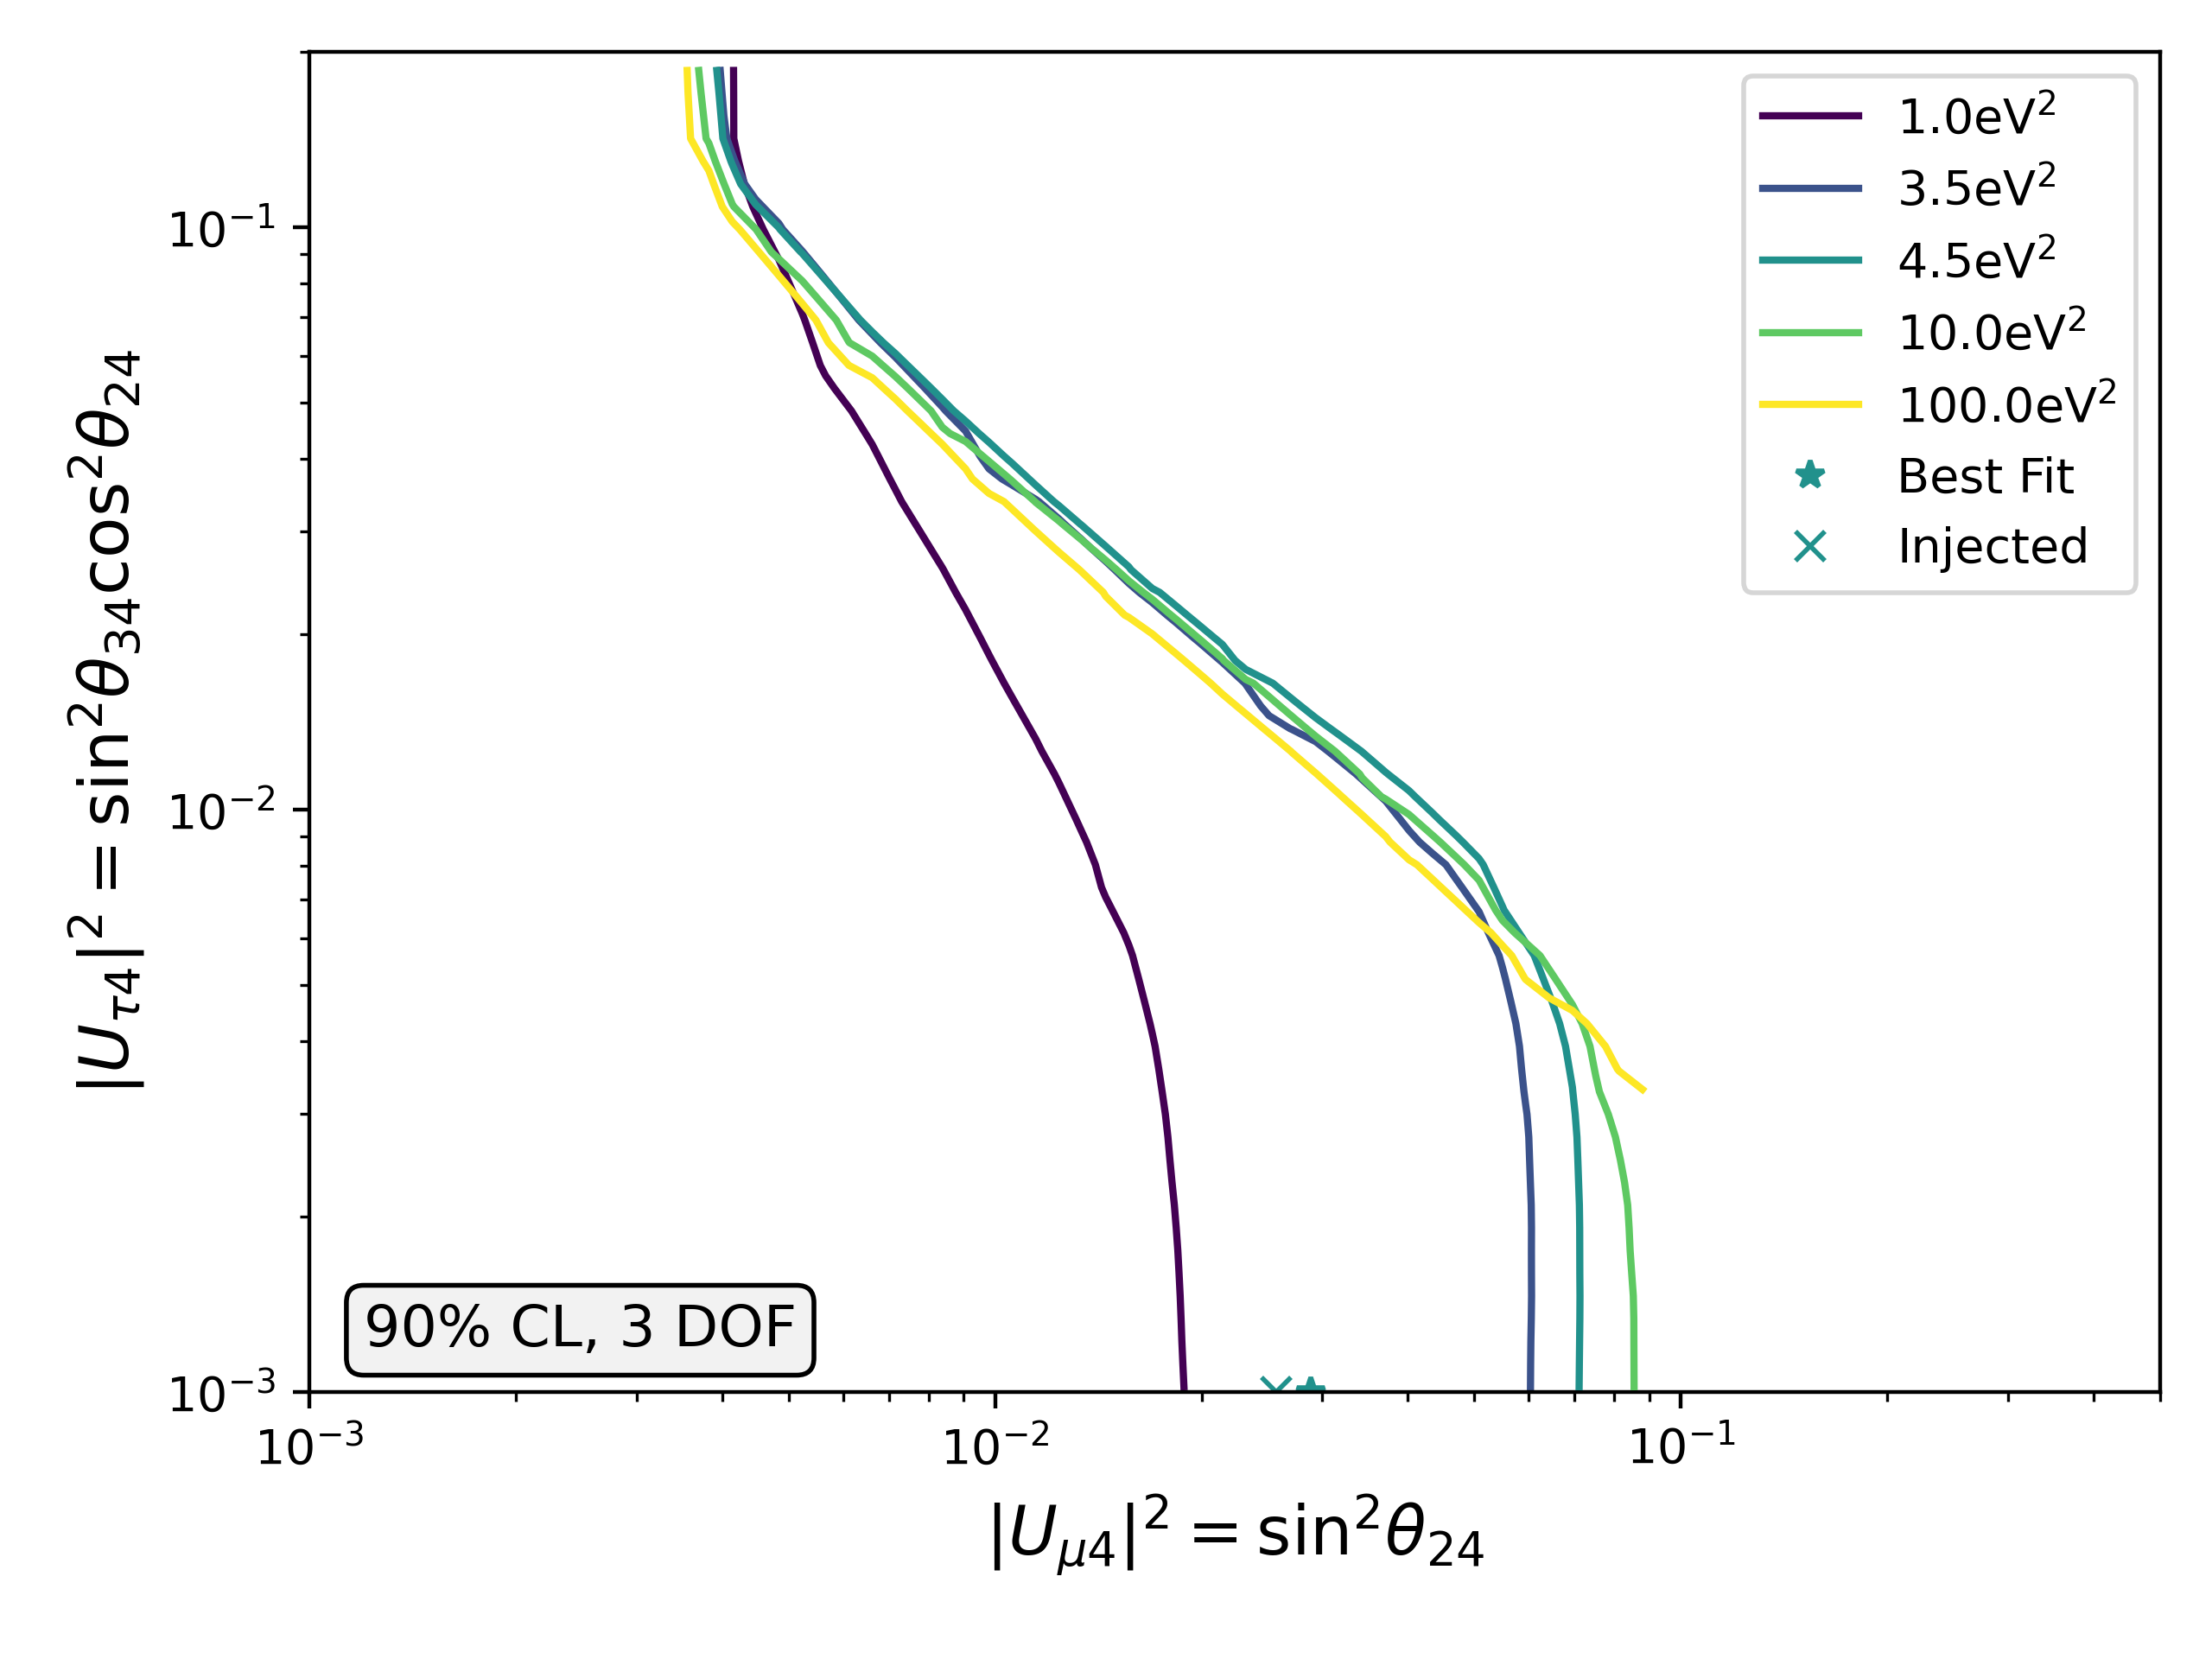
\includegraphics[width=0.45\linewidth]{figures/inject_recover_RealIR_9_sterile_4_cl0.9_dof3.png}
    \caption{To be added later}
\end{figure}

\section{Unblinding Procedure}

\begin{figure}
    \centering
    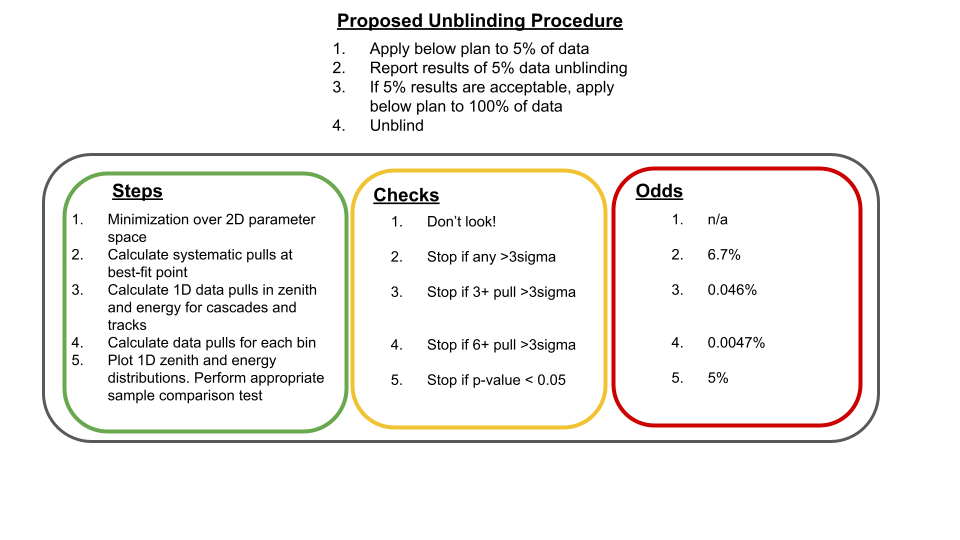
\includegraphics[width=0.7\linewidth]{figures/unblinding.png}
    \caption{The unblinding procedure used in this analysis and expected probabilities of satisfying the stop condition.}\label{fig:unblind}
\end{figure}

The unblinding procedure used in this analysis is shown in Figure~\ref{fig:unblind}. 
First, a full 3D fit-scan is applied while fitting to only 5\% of the full dataset. 
No best fit parameters or likelihoods are reported. 
At the best fit point, if any nuisance parameters have a fit value more than $3\sigma$ away from their central values, we stop. 
Then we count the number of bins whose best fit values are more than $3\sigma$ away from their expected value; if more than 3 satisfy this condition, we stop. 


\section{Results}

\section{Conclusions}

\end{document}